% !TeX document-id = {d11ec887-967f-47dd-b58f-2345d0feed09}
% !TEX TS-program = XeLaTeX
% Command for running this example (needs latexmkrc file):
%    latexmk -bibtex -pdf main.tex

%	نمونه پایان‌نامه آماده شده با استفاده از کلاس tehran-thesis، نگارش 1
%	سینا ممکن، دانشگاه تهران 
%	https://github.com/sinamomken/tehran-thesis
%	گروه پارسی‌لاتک
%	http://www.parsilatex.com
%	این نسخه، بر اساس نسخه‌ 0.1 از کلاس IUST-Thesis آقای محمود امین‌طوسی آماده شده است.
%        http://profsite.sttu.ac.ir/mamintoosi

%----------------------------------------------------------------------------------------------
% اگر قصد نوشتن پروژه کارشناسی را دارید، در خط زیر به جای msc، کلمه bsc و اگر قصد نوشتن رساله دکترا را دارید، کلمه phd را قرار دهید. کلیه تنظیمات لازم، به طور خودکار، اعمال می‌شود.

% اگر مایلید پایان‌نامه شما دورو باشد به جای oneside در خط زیر از twoside استفاده کنید.

% برای حاشیه‌نویسی و کم کردن صفحات ابتدایی، گزینه draft را وارد و برای نسخه نهایی آن را حذف کنید.
\documentclass[twoside,openany,msc]{tehran-thesis} % draft

% فایل commands.tex را مطالعه کنید؛ چون دستورات مربوط به فراخوانی بسته‌ها، فونت و دستورات خاص در این فایل قرار دارد.
% در این فایل، دستورها و تنظیمات مورد نیاز، آورده شده است.
%-------------------------------------------------------------------------------------------------------------------
% دستوراتی که پوشه پیش‌فرض زیرفایل‌های tex را مشخص می‌کند.
%\makeatletter
%\def\input@path{{./tex/}}
%\makeatother
% در ورژن جدید زی‌پرشین برای تایپ متن‌های ریاضی، این سه بسته، حتماً باید فراخوانی شود

\usepackage[top=40mm, bottom=40mm, left=25mm, right=35mm, headheight=15pt]{geometry}
% رفع خطای UseMathForPositioningText در bidi برای جداول فارسی
\makeatletter
\providecommand{\UseMathForPositioningText}{}
\makeatother
% بسته‌‌ای برای ظاهر شدن شکل‌ها و تعیین آدرس تصاویر
\usepackage[final]{graphicx}
\graphicspath{{./img/}}
% بسته‌های مورد نیاز برای نوشتن کدها، رنگ‌آمیزی آنها و تعیین پوشهٔ کدها
\usepackage[final]{listings}
\usepackage[usenames,dvipsnames,svgnames,table]{xcolor}
\lstset{inputpath=./code/}
% بسته‌ای برای رسم کادر
\usepackage{framed} 
% بسته‌‌ای برای چاپ شدن خودکار تعداد صفحات در صفحه «معرفی پایان‌نامه»
\usepackage{lastpage}
% بسته‌ٔ لازم برای: ۱. تغییر شماره‌گذاری صفحات پیوست. ۲. تصحیح باگ آدرس وب حاوی '%' در مراجع
\usepackage{etoolbox}
% بسته برای فرمول‌های چندخطی (split، align، …) و تعریف قضیه
\usepackage{amsmath}
\usepackage{amsthm}

%%%%%%%%%%%%%%%%%%%%%%%%%%%%%%%%%%%%
%%% دستورات وابسته به استیل مراجع:
%% اگر از استیل‌های natbib (plainnat-fa، asa-fa، chicago-fa) استفاده می‌کنید، خط زیر را فعال و بعدی‌اش را غیرفعال کنید.
%\usepackage{natbib}
%\newcommand{\citelatin}[1]{\cite{#1}\LTRfootnote{\citeauthor*{#1}}}
%\newcommand{\citeplatin}[1]{\citep{#1}\LTRfootnote{\citeauthor*{#1}}}
%% اگر از سایر استیل‌ها استفاده می‌کنید، خط بالا را غیرفعال و خط‌های زیر را فعال کنید.
\let\citep\cite
\let\citelatin\cite
\let\citeplatin\cite
%%%%%%%%%%%%
% بررسی حالت پیش نویس
\usepackage{ifdraft}
\ifdraft
{%
	% بسته‌ٔ ایجاد لینک‌های رنگی با امکان جهش
	\usepackage[unicode=true,pagebackref=true,
colorlinks,linkcolor=blue,citecolor=blue,final]{hyperref}
	%\usepackage{todonotes}
	\usepackage[firstpage]{draftwatermark}
	\SetWatermarkText{برچسب}
	\SetWatermarkScale{1.2}
}
{ 
	\usepackage[pagebackref=false,colorlinks,
	linkcolor=blue,citecolor=blue,urlcolor=blue]{hyperref}
	%\usepackage[disable]{todonotes} % final without TODOs
}

\usepackage[obeyDraft]{todonotes}
\setlength{\marginparwidth}{2cm}

% تعیین مشخصات فایل PDF
\hypersetup{
pdftitle={My Thesis},
pdfauthor={Sina Momken},
pdfsubject={Master Thesis},
pdfkeywords={keywords},
pdfdirection={R2L}
}
%%%%%%%%%%%%
%%% تصحیح باگ: اگر در مراجع، آدرس وب حاوی '%' بوده و pagebackref فعال باشد، دستورات زیر باید بیایند:
%% برای استیل‌های natbib مثل plainnat-fa، asa-fa، chicago-fa
\makeatletter
\let\ORIG@BR@@lbibitem\BR@@lbibitem
\apptocmd\ORIG@BR@@lbibitem{\endgroup}{}{}
\def\BR@@lbibitem{\begingroup\catcode`\%=12 \ORIG@BR@@lbibitem}
\makeatother
%% برای سایر استیل‌ها
\makeatletter
\let\ORIG@BR@@bibitem\BR@@bibitem
\apptocmd\ORIG@BR@@bibitem{\endgroup}{}{}
\def\BR@@bibitem{\begingroup\catcode`\%=12 \ORIG@BR@@bibitem}
\makeatother
%%%%%%%%%%%%%%%%%%%%%%%%%%%%%%%%%%%%

% بسته‌ لازم برای تنظیم سربرگ‌ها
\usepackage{fancyhdr}
%\usepackage{enumitem}
\usepackage{setspace}
% بسته‌های لازم برای نوشتن الگوریتم
\usepackage{algorithm}
\usepackage{algorithmic}
\usepackage{algorithm}
\usepackage{caption}
% \usepackage{algpseudocode}

% بسته‌های لازم برای رسم بهتر جداول
\usepackage{tabulary}
\usepackage{tabularx}
% بسته‌های لازم برای رسم تنظیم بهتر شکل‌ها و زیرشکل‌ها
\usepackage[export]{adjustbox}
\usepackage{subfigure}
\usepackage[subfigure]{tocloft}
% بسته‌ای برای رسم نمودارها و نیز صفحه مالکیت اثر
\usepackage{tikz}
% بسته‌ای برای ظاهر شدن «مراجع» و «نمایه» در فهرست مطالب
\usepackage[nottoc]{tocbibind}
% دستورات مربوط به ایجاد نمایه
\usepackage{makeidx}
\makeindex
%%% بسته ایجاد واژه‌نامه با xindy
\usepackage[xindy,acronym,nonumberlist=true]{glossaries}

% بسته زیر باگ ناشی از فراخوانی بسته‌های زیاد را برطرف می‌کند.
\usepackage{morewrites}
%%%%%%%%%%%%%%%%%%%%%%%%%%
% فراخوانی بسته زی‌پرشین (باید آخرین بسته باشد)، تعریف قلم فارسی و انگلیسی و مکان قلم‌ها
\usepackage[extrafootnotefeatures]{xepersian}
\settextfont[Path={./font/}, BoldFont={IRLotusICEE_Bold.ttf}, BoldItalicFont={IRLotusICEE_BoldIranic.ttf}, ItalicFont={IRLotusICEE_Iranic.ttf},Scale=1.2]{IRLotusICEE.ttf}

% LiberationSerif or FreeSerif as free equivalents of Times New Roman
\setlatintextfont[Path={./font/}, BoldFont={LiberationSerif-Bold.ttf}, BoldItalicFont={LiberationSerif-BoldItalic.ttf}, ItalicFont={LiberationSerif-Italic.ttf},Scale=1]{LiberationSerif-Regular.ttf}
%%%%%%%%%%%%%%%%%%%%%%%%%%
% چنانچه می‌خواهید اعداد در فرمول‌ها، انگلیسی باشد، خط زیر را غیرفعال کنید
\setdigitfont[Path={./font/}, Scale=1.2]{IRLotusICEE.ttf}
%%%%%%%%%%%%%%%%%%%%%%%%%%
% تعریف قلم‌های فارسی و انگلیسی اضافی برای استفاده در بعضی از قسمت‌های متن
\defpersianfont\titlefont[Path={./font/}, Scale=1]{IRTitr.ttf}
\setiranicfont[Path={./font/}, Scale=1.3]{IRLotusICEE_Iranic.ttf}				% ایرانیک، خوابیده به چپ
% \defpersianfont\nastaliq[Scale=1.2]{IranNastaliq}
\setmathsfdigitfont[Path={./font/}]{IRTitr.ttf}
%%%%%%%%%%%%%%%%%%%%%%%%%%
% راستچین شدن todonotes
\presetkeys{todonotes}{align=right,textdirection=righttoleft}{}
\makeatletter
\providecommand\@dotsep{5}
\def\listtodoname{فهرست کارهای باقیمانده}
\def\listoftodos{\noindent{\Large\vspace{10mm}\textbf{\listtodoname}}\@starttoc{tdo}}
\renewcommand{\@todonotes@MissingFigureText}{شکل}
\renewcommand{\@todonotes@MissingFigureUp}{شکل}
\renewcommand{\@todonotes@MissingFigureDown}{جاافتاده}
\makeatother
% دستوری برای حذف کلمه «چکیده»
\providecommand{\abstractname}{}
% دستوری برای حذف کلمه «abstract»
%\renewcommand{\latinabstract}{}
% دستوری برای تغییر نام کلمه «اثبات» به «برهان»
\renewcommand\proofname{\textbf{برهان}}
% دستوری برای تغییر نام کلمه «کتاب‌نامه» به «مراجع»
\renewcommand{\bibname}{مراجع}
% دستوری برای تعریف واژه‌نامه انگلیسی به فارسی
\newcommand\persiangloss[2]{#1\dotfill\lr{#2}\\}
% دستوری برای تعریف واژه‌نامه فارسی به انگلیسی 
\newcommand\englishgloss[2]{#2\dotfill\lr{#1}\\}
% تعریف دستور جدید «\پ» برای خلاصه‌نویسی جهت نوشتن عبارت «پروژه/پایان‌نامه/رساله»
\newcommand{\پ}{پروژه/پایان‌نامه/رساله }

%\newcommand\BackSlash{\char`\\}

%%%%%%%%%%%%%%%%%%%%%%%%%%
\SepMark{-}

% تعریف و نحوه ظاهر شدن عنوان قضیه‌ها، تعریف‌ها، مثال‌ها و ...
\theoremstyle{definition}
\newtheorem{definition}{تعریف}[section]
\theoremstyle{theorem}
\newtheorem{theorem}[definition]{قضیه}
\newtheorem{lemma}[definition]{لم}
\newtheorem{proposition}[definition]{گزاره}
\newtheorem{corollary}[definition]{نتیجه}
\newtheorem{remark}{توجه}[section]
\theoremstyle{definition}
\newtheorem{example}{مثال}[section]

%\renewcommand{\theequation}{\thechapter-\arabic{equation}}
%\def\bibname{مراجع}
\numberwithin{algorithm}{chapter}
\def\listalgorithmname{}
\def\listfigurename{فهرست تصاویر}
\def\listtablename{فهرست جداول}

%%%%%%%%%%%%%%%%%%%%%%%%%%%%
%%% دستورهایی برای سفارشی کردن سربرگ صفحات:
%\newcommand{\SetHeader}[1]{
% دستور زیر معادل با گزینه twoside است.
%\csname@twosidetrue\endcsname
\pagestyle{fancy}
%% دستورات زیر سبک صفحات fancy را تغییر می‌دهد:
% O=Odd, E=Even, L=Left, R=Right
% در صورت oneside بودن، عنوان فصل، سمت چپ ظاهر می‌شود.
\fancyhead{}
\fancyhead[OL]{\small\leftmark}
\fancyhead[ER]{\small\leftmark}
% شکل‌دهی شماره و عنوان فصل در سربرگ
%\renewcommand{\chaptermark}[1]{\markboth{\thechapter-\ #1}{}}
%}
%%%%%%%%%%%%%%%%%%%%%%%%%%%%
%\def\MATtextbaseline{1.5}
%\renewcommand{\baselinestretch}{\MATtextbaseline}
\doublespacing
%%%%%%%%%%%%%%%%%%%%%%%%%%%%%
% دستوراتی برای اضافه کردن کلمه «فصل» در فهرست مطالب

\newlength\mylenprt
\newlength\mylenchp
\newlength\mylenapp

\renewcommand\cftpartpresnum{\partname~}
\renewcommand\cftchappresnum{\chaptername~}
\renewcommand\cftchapaftersnum{:}

\settowidth\mylenprt{\cftpartfont\cftpartpresnum\cftpartaftersnum}
\settowidth\mylenchp{\cftchapfont\cftchappresnum\cftchapaftersnum}
\settowidth\mylenapp{\cftchapfont\appendixname~\cftchapaftersnum}
\addtolength\mylenprt{\cftpartnumwidth}
\addtolength\mylenchp{\cftchapnumwidth}
\addtolength\mylenapp{\cftchapnumwidth}

\setlength\cftpartnumwidth{\mylenprt}
\setlength\cftchapnumwidth{\mylenchp}	

\makeatletter
{\def\thebibliography#1{\chapter*{\refname\@mkboth
   {\uppercase{\refname}}{\uppercase{\refname}}}\list
   {\lr{[\@arabic\c@enumiv]}}{\settowidth\labelwidth{\lr{[#1]}}
   \rightmargin\labelwidth
   \advance\rightmargin\labelsep
   \advance\rightmargin\bibindent
   \itemindent -\bibindent

   \listparindent \itemindent
   \parsep \z@
   \usecounter{enumiv}}
   \def\newblock{}
   \sloppy
   \sfcode`\.=1000\relax}}
   
%اگر مایلید در شماره گذاری حرفی و ابجد به جای آ از الف استفاده شود دستورات زیر را فعال کنید.   
%\def\@Abjad#1{%
%  \ifcase#1\or الف\or ب\or ج\or د%
%           \or هـ\or و\or ز\or ح\or ط%
%           \or ی\or ک\or ل\or م\or ن%
%           \or س\or ع\or ف\or ص%
%           \or ق\or ر\or ش\or ت\or ث%
%            \or خ\or ذ\or ض\or ظ\or غ%
%            \else\@ctrerr\fi}
%
% \def\abj@num@i#1{%
%   \ifcase#1\or الف\or ب\or ج\or د%
%            \or هـ‍\or و\or ز\or ح\or ط\fi

%   \ifnum#1=\z@\abjad@zero\fi}   
%  
%   \def\@harfi#1{\ifcase#1\or الف\or ب\or پ\or ت\or ث\or

% ج\or چ\or ح\or خ\or د\or ذ\or ر\or ز\or ژ\or س\or ش\or ص\or ض\or ط\or ظ\or ع\or غ\or

% ف\or ق\or ک\or گ\or ل\or م\or ن\or و\or ه\or ی\else\@ctrerr\fi}

%
\makeatother

%%% امکان درج کد در سند
% در این قسمت رنگ، قلم و قالب‌بندی قسمت‌های مختلف یک کد تعیین می‌شود. 
\lstdefinestyle{myStyle}{
	basicstyle=\ttfamily, % whole listing /w verbatim font
	keywordstyle=\color{blue}\bfseries, % bold black keywords
	identifierstyle=, % nothing happens
	commentstyle=\color{LimeGreen}, % green comments
	stringstyle=\ttfamily\color{red}, % red typewriter font for strings
	showstringspaces=false % no special string spaces
	breaklines=true,
	breakatwhitespace=false,
	numbers=right, % line number formats
	numberstyle=\footnotesize\lr,
	numbersep=-10pt,
	frame=single,
	captionpos=b,
	captiondirection=RTL
}
\lstset{style=myStyle} % command to set default style
\def\lstlistingname{\rl{برنامه}}


% for numbering subsubsections
\setcounter{secnumdepth}{3}
%to include subsubsections in the table of contents
\setcounter{tocdepth}{3}


% تنظیمات و تعاریف واژه‌نامه و اختصارات
%%% تنظیمات مربوط به بسته  glossaries
%%% تعریف استایل برای واژه نامه فارسی به انگلیسی، در این استایل واژه‌های فارسی در سمت راست و واژه‌های انگلیسی در سمت چپ خواهند آمد. از حالت گروه ‌بندی استفاده می‌کنیم، 
%%% یعنی واژه‌ها در گروه‌هایی به ترتیب حروف الفبا مرتب می‌شوند، مثلا:
%%% الف
%%% افتصاد ................................... Economy
%%% اشکال ........................................ Failure
%%% ش
%%% شبکه ...................................... Network
\newglossarystyle{myFaToEn}{%
	\renewenvironment{theglossary}{\begin{multicols}{2}\setlength{\parskip}{0pt}\setlength{\parindent}{0pt}}{\end{multicols}}
	% برای جلوگیری از خطوط خالی و کاراکترهای نامعتبر در گروه‌بندی فارسی
	\renewcommand*{\glsgroupskip}{}
	\renewcommand*{\glsgroupheading}[1]{}
	\renewcommand*{\glossentry}[2]{\noindent\glsentryname{##1}\dotfill\space \glsentrytext{##1}\par}
}

%% % تعریف استایل برای واژه نامه انگلیسی به فارسی، در این استایل واژه‌های فارسی در سمت راست و واژه‌های انگلیسی در سمت چپ خواهند آمد. از حالت گروه ‌بندی استفاده می‌کنیم، 
%% % یعنی واژه‌ها در گروه‌هایی به ترتیب حروف الفبا مرتب می‌شوند، مثلا:
%% % E
%%% Economy ............................... اقتصاد
%% % F
%% % Failure................................... اشکال
%% %N
%% % Network ................................. شبکه

\newglossarystyle{myEntoFa}{%
	%%% این دستور در حقیقت عملیات گروه‌بندی را انجام می‌دهد. بدین صورت که واژه‌ها در بخش‌های جداگانه گروه‌بندی می‌شوند، 
	%%% عنوان بخش همان نام حرفی است که هر واژه در آن گروه با آن شروع شده است. 
	\renewenvironment{theglossary}{\begin{multicols}{2}\setlength{\parskip}{0pt}\setlength{\parindent}{0pt}}{\end{multicols}}
	\renewcommand*{\glsgroupskip}{}
	\renewcommand*{\glsgroupheading}[1]{}
	%%% در این دستور نحوه نمایش واژه‌ها می‌آید. در این جا واژه فارسی در سمت راست و واژه انگلیسی در سمت چپ قرار داده شده است، و بین آن با نقطه پر می‌شود. 
	\renewcommand*{\glossentry}[2]{\noindent\glsentrytext{##1}\dotfill\space \glsentryname{##1}\par}
}

%%% تعیین استایل برای فهرست اختصارات
\newglossarystyle{myAbbrlist}{%
	%%% این دستور در حقیقت عملیات گروه‌بندی را انجام می‌دهد. بدین صورت که اختصارات‌ در بخش‌های جداگانه گروه‌بندی می‌شوند، 
	%%% عنوان بخش همان نام حرفی است که هر اختصار در آن گروه با آن شروع شده است. 
	\renewenvironment{theglossary}{}{}
	\renewcommand*{\glsgroupskip}{\vskip 10mm}
	\renewcommand*{\glsgroupheading}[1]{\begin{LTR} \subsection*{\glsgetgrouptitle{##1}} \end{LTR}}
	%%% در این دستور نحوه نمایش اختصارات می‌آید. در این جا حالت کوچک اختصار در سمت چپ و حالت بزرگ در سمت راست قرار داده شده است، و بین آن با نقطه پر می‌شود. 
	\renewcommand*{\glossentry}[2]{\noindent\Glsentrylong{##1}\dotfill\space \glsentrytext{##1} 
		
	}
	%%% تغییر نام محیط abbreviation به فهرست اختصارات
	\renewcommand*{\acronymname}{\rl{فهرست اختصارات}}
}

%%% برای اجرا xindy بر روی فایل .tex و تولید واژه‌نامه‌ها و فهرست اختصارات و فهرست نمادها یکسری  فایل تعریف شده است.‌ Latex داده های مربوط به واژه نامه و .. را در این 
%%%  فایل‌ها نگهداری می‌کند. مهم‌ترین option‌ این قسمت این است که 
%%% عنوان واژه‌نامه‌ها و یا فهرست اختصارات و یا فهرست نمادها را می‌توانید در این‌جا مشخص کنید. 
%%% در این جا عباراتی مثل glg، gls، glo و ... پسوند فایل‌هایی است که برای xindy بکار می‌روند. 
\newglossary[glg]{english}{gls}{glo}{واژه‌نامه انگلیسی به فارسی}
\newglossary[blg]{persian}{bls}{blo}{واژه‌نامه فارسی به انگلیسی}
\makeglossaries
\glsdisablehyper
%%% تعاریف مربوط به تولید واژه نامه و فهرست اختصارات و فهرست نمادها
%%%  در این فایل یکسری دستورات عمومی برای وارد کردن واژه‌نامه آمده است.
%%%  به دلیل این‌که قرار است این دستورات پایه‌ای را بازنویسی کنیم در این‌جا تعریف می‌کنیم. 
\let\oldgls\gls
\let\oldglspl\glspl

\makeatletter

\renewrobustcmd*{\gls}{\@ifstar\@msgls\@mgls}
\newcommand*{\@mgls}[1] {\ifthenelse{\equal{\glsentrytype{#1}}{english}}{\oldgls{#1}\glsuseri{f-#1}}{\lr{\oldgls{#1}}}}
\newcommand*{\@msgls}[1]{\ifthenelse{\equal{\glsentrytype{#1}}{english}}{\glstext{#1}\glsuseri{f-#1}}{\lr{\glsentryname{#1}}}}

\renewrobustcmd*{\glspl}{\@ifstar\@msglspl\@mglspl}
\newcommand*{\@mglspl}[1] {\ifthenelse{\equal{\glsentrytype{#1}}{english}}{\oldglspl{#1}\glsuseri{f-#1}}{\oldglspl{#1}}}
\newcommand*{\@msglspl}[1]{\ifthenelse{\equal{\glsentrytype{#1}}{english}}{\glsplural{#1}\glsuseri{f-#1}}{\glsentryplural{#1}}}

\makeatother

\newcommand{\newword}[4]{
	\newglossaryentry{#1}     {type={english},name={\lr{#2}},plural={#4},text={#3},description={}}
	\newglossaryentry{f-#1} {type={persian},name={#3},text={\lr{#2}},description={}}
}

%%% بر طبق این دستور، در اولین باری که واژه مورد نظر از واژه‌نامه وارد شود، پاورقی زده می‌شود. 
\defglsentryfmt[english]{\glsgenentryfmt\ifglsused{\glslabel}{}{\LTRfootnote{\glsentryname{\glslabel}}}}

%%% بر طبق این دستور، در اولین باری که واژه مورد نظر از فهرست اختصارات وارد شود، پاورقی زده می‌شود. 
\defglsentryfmt[acronym]{\glsentryname{\glslabel}\ifglsused{\glslabel}{}{\footnote{\glsentrydesc{\glslabel}}}}


%%%%%% ============================================================================================================

%%============================ دستور برای قرار دادن فهرست اختصارات 
\newcommand{\printabbreviation}{
	%\cleardoublepage
	%\phantomsection
	\baselineskip=.75cm
	%% با این دستور عنوان فهرست اختصارات به فهرست مطالب اضافه می‌شود. 
	\addcontentsline{toc}{chapter}{فهرست اختصارات}
	\setglossarystyle{myAbbrlist}
	%\begin{LTR}
		\Oldprintglossary[type=acronym]	
	%\end{LTR}
	\clearpage
}%

\newcommand{\printacronyms}{\printabbreviation}
%%% در این جا محیط هر دو واژه نامه را باز تعریف کرده ایم، تا اولا مشکل قرار دادن صفحه اضافی را حل کنیم، ثانیا عنوان واژه نامه ها را با دستور addcontentlist وارد فهرست مطالب کرده ایم.
\let\Oldprintglossary\printglossary
% جلوگیری از رفتار chapter* (و صفحه خالی در حالت twoside) برای عنوان واژه‌نامه‌ها
\renewcommand*{\glossarysection}[2][]{\section*{#2}}
\renewcommand{\printglossary}{
	\let\appendix\relax
	% جلوگیری از ایجاد صفحه خالی زوج قبل از عنوان واژه‌نامه در حالت دورو
	\let\cleardoublepage\clearpage
	%% همه مدخل‌ها را حتی اگر در متن فراخوانی نشده باشند، به واژه‌نامه اضافه کن
	\glsaddall
	%% تنظیم کننده فاصله بین خطوط در این قسمت
	% \clearpage  % حذف شد تا صفحه خالی قبل از واژه‌نامه ایجاد نشود
	%\phantomsection
	%% حالت دوستونه در خود استایل واژه‌نامه مدیریت می‌شود (multicols)
	%% با این دستور عنوان واژه‌نامه به فهرست مطالب اضافه می‌شود. 
	\addcontentsline{toc}{chapter}{واژه نامه فارسی به انگلیسی}
	\setglossarystyle{myFaToEn}
	\Oldprintglossary[type=persian]
	\clearpage
	%\phantomsection
	%% با این دستور عنوان واژه‌نامه به فهرست مطالب اضافه می‌شود. 
	\addcontentsline{toc}{chapter}{واژه نامه انگلیسی به فارسی}
	\setglossarystyle{myEntoFa}
	\Oldprintglossary[type=english]	
}%
%%%%%%

%%%% A

\newword{Artificial neural networks}{Artificial neural network}{شبکه‌های عصبی مصنوعی}{شبکه‌های عصبی مصنوعی}

\newword{Dendrites}{Dendrites}{دندریت‌ها}{دندریت‌ها}

\newword{Cell body}{Cell body}{جسم سلولی}{جسم سلولی}


\newword{Axon}{Axon}{آکسون}{آکسون}

\newword{Synapse}{Synapse}{سیناپس}{سیناپس}

\newword{Rectified Linear Unit (RELU)}{Rectified Linear Unit (RELU)}{واحد یکسو شده‌ی خطی}{واحد یکسو شده‌ی خطی}

\newword{Sigmoid}{Sigmoid}{سیگموئید}{سیگموئید}

\newword{Classification}{Classification}{طبقه‌بندی}{طبقه‌بندی}

\newword{MLP}{Multi-Layer perceptron (MLP)}{پرسپترون چند لایه}{پرسپترون چند لایه}

\newword{Bias}{Bias}{پیش‌قدر}{پیش‌قدر}

\newword{Class}{Class}{رده}{رده}

\newword{CE}{Cross-entropy}{آنتروپی متقاطع}{آنتروپی متقاطع}

\newword{SSE}{Sum of squares errors (SSE)}{مجموع مربعات خطاها}{مجموع مربعات خطاها}

\newword{HT}{Hyperbolic Tangent}{تانژانت هیپربولیک}{تانژانت هیپربولیک}

\newword{BP}{Back propagation}{پس انتشار}{پس انتشار}

\newword{Likelihood}{Likelihood}{درست‌نمایی}{درست‌نمایی}

\newword{Categorical distribution}{Categorical distribution}{توزیع دسته‌ای}{توزیع دسته‌ای}

\newword{Indicator}{Indicator}{نشان‌گر}{نشان‌گر}

\newword{Prior}{Prior}{پیشین}{پیشین}

\newword{Posterior distribution}{Posterior distribution}{توزیع پسین}{توزیع پسین}

\newword{Evidence}{Evidence}{شواهد}{شواهد}

\newword{Improper}{Improper}{ناسره}{ناسره}

\newword{Conjugate}{Conjugate}{مزدوج}{مزدوج}

\newword{MAP}{Maximum a posteriori (MAP)}{بیشینه احتمال پسین}{بیشینه احتمال پسین}

\newword{NC}{Natural conjugate}{مزدوج طبیعی}{مزدوج طبیعی}

\newword{SS}{Sufficient Statistic}{آماره بسنده}{آماره بسنده}

\newword{SICS}{Scaled inverse chi-squared}{کای دو معکوس مقیاس شده}{کای دو معکوس مقیاس شده}

\newword{Semi-conjugate}{Semi-conjugate}{نیمه مزدوج}{نیمه مزدوج}

\newword{Non-conjugate}{Non-conjugate}{نامزدوج}{نامزدوج}

\newword{BLR}{Bayesian logistic regression}{رگرسیون لجستیک بیزی}{رگرسیون لجستیک بیزی}

\newword{Noninformative}{Noninformative}{ناآگاهی بخش}{ناآگاهی بخش}

\newword{Jeffryes}{Jeffreys’ prior}{پیشین جفریز}{پیشین جفریز}

\newword{Fisher information}{Fisher information}{اطلاع فیشر}{اطلاع فیشر}

\newword{BNNs}{Bayesian neural networks (BNNs)}{شبکه‌های عصبی بیزی}{شبکه‌های عصبی بیزی}

\newword{Overfitting}{Overfitting}{بیش‌برازش}{بیش‌برازش}

\newword{Ensemble learning}{Ensemble learning}{یادگیری ترکیبی}{یادگیری ترکیبی}

\newword{Bagging}{Bagging}{دسته‌بندی}{دسته‌بندی}


\newword{Bioinformatics}{Bioinformatics}{بیوانفورماتیک}{بیوانفورماتیک}

\newword{Robustness}{Robustness}{استواری}{استواری}

\newword{MCMC}{Markov chain monte carlo (MCMC)}{زنجیره مارکوف مونت کارلو}{زنجیره مارکوف مونت کارلو}

\newword{VB}{Variational Bayes (VB)}{بیز تغییراتی}{بیز تغییراتی}

\newword{Accuracy}{Accuracy}{دقت}{دقت}

\newword{F-measure}{F-measure}{$\text{\lr{F}}$-اندازه}{$\text{\lr{F}}$-اندازه}

\newword{Jaccard score}{Jaccard score}{نمره یاکارد}{نمره یاکارد}

\newword{Classifier}{Classifier}{طبقه‌بند}{طبقه‌بند}

\newword{ROC}{Receiver Operating Characteristic (ROC)}{منحنی مشخصه عامل گیرنده}{منحنی مشخصه عامل گیرنده}

\newword{AUC}{Area under the ROC Curve}{AUC}{AUC}

\newword{LA}{Laplace approximation}{تقریب لاپلاس}{تقریب لاپلاس}

\newword{Ergodic}{Ergodic}{ارگودیک}{ارگودیک}

\newword{Metropolis-Hastings}{Metropolis-Hastings}{متروپولیس-هستینگر}{متروپولیس-هستینگز}

\newword{Gibbs sampler}{Gibbs sampler}{نمونه‌بردار گیبز}{نمونه‌بردار گیبز}

\newword{GMM}{Gaussian mixture models}{مدل‌های آمیخته گاوسی}{مدل‌های آمیخته گاوسی}

\newword{EM}{Expectation maximization}{بیشینه‌سازی امید ریاضی}{بیشینه‌سازی امید ریاضی}

\newword{IW}{Inverse wishart}{ویشارت معکوس}{ویشارت معکوس}

\newword{Dir}{Dirichlet}{دیریکله}{دیریکله}

\newword{Trace}{Trace}{اثر}{اثر}

\newword{RW}{Random walk}{گام‌برداری تصادفی}{گام‌برداری تصادفی}

\newword{Proposal distribution}{Proposal distribution}{توزیع پیشنهاده}{توزیع پیشنهاده}

\newword{Irreducible}{Irreducible}{تحویل‌ناپذیر}{تحویل‌ناپذیر}

\newword{Aperiodic}{Aperiodic}{نامتناوب}{نامتناوب}

\newword{Recurrent}{Recurrent}{بازگشتی}{بازگشتی}

\newword{State}{State}{حالت}{حالت}

\newword{Hessian}{Hessian}{هسین}{هسین}

\newword{Burn-in}{Burn-in}{داغیدن}{داغیدن}

\newword{AC}{Autocorrelation}{خود همبستگی}{خود همبستگی}

\newword{AR}{Acceptance rate}{نرخ پذیرش}{نرخ پذیرش}

\newword{KLD}{Kullback-Leibler divergence}{واگرایی کولبک-لیبلر}{واگرایی کولبک-لیبلر}

\newword{System Biology}{System Biology}{سیستم‌های بیولوژیکی}{سیستم‌های بیولوژیکی}

\newword{Sequencing}{Senquencing}{توالی‌یابی}{توالی‌یابی}

\newword{Genome-Wide Association Study}{Genome-Wide Association Study}{حوزه مطالعهٔ ارتباطات گسترده ژنوم}{حوزه مطالعهٔ ارتباطات گسترده ژنوم}

\newword{Single Nucleotide Polymorphism}{Single Nucleotide Polymorphism}{تک نوکلئوتید چندریختی}{تک نوکلئوتید چندریختی}

\newword{Allele}{Allele}{آلل}{آلل‌ها}

\newword{Admix}{Admix}{مخلوط}{مخلوط}

\newword{Markov chain Monte Carlo(MCMC)}{Markov chain Monte Carlo(MCMC)}{زنجیره مارکوف مونت کارلو}{زنجیره مارکوف مونت کارلو}

\newword{Admixture}{Admixture}{مخلوطی}{مخلوطی}

\newword{Epistasis}{Epistasis}{اپیستازیس}{اپیستازیس}

\newword{Disease Risk}{Disease Risk}{خطر ابتلا به بیماری}{خطر ابتلا به بیماری}

\newword{Personalized Medicine}{Personalized Medicine}{ شخصی سازی دارو}{ شخصی سازی دارو}

\newword{Natural Selection}{Natural Selection}{انتخاب طبیعی}{انتخاب طبیعی}


%\newword{Personalized Medicine}{Personalized Medicine}{پزشکی فردی}{پزشکی فردی}

\newword{Diabet Type 1}{Diabet Type 1}{دیابت نوع ۱}{دیابت نوع ۱}

\newword{Diabet Type 2}{Diabet Type 2}{دیابت نوع ۲}{دیابت نوع ۲}

\newword{Intron}{Intron}{اینترون}{اینترون}

\newword{Breast Cancer}{Breast Cancer}{سرطان سینه}{سرطان سینه}

\newword{Prostate Cancer}{Prostate Cancer}{سرطان پروستات}{سرطان پروستات}

\newword{Marker}{Marker}{نشانگر}{نشانگر}

\newword{Parkinson}{Parkinson}{پارکینسون}{پارکینسون}

\newword{Bipolar}{Bipolar}{دوقطبی}{دوقطبی}

\newword{Schizophrenia}{Schizophrenia}{ اسکیزوفرنی}{ اسکیزوفرنی}

\newword{Principal Component Analysis}{Principal Component Analysis}{تحلیل مؤلفه های اصلی}{تحلیل مؤلفه های اصلی}

\newword{Mixture Model}{Mixture Model}{مدل آمیخته}{مدل آمیخته}

\newword{Minor Allele Frequency (MAF)}{Minor Allele Frequency (MAF)}{فراوانی آلل کوچک تر}{فراوانی آلل کوچک تر}

\newword{Deoxyribonucleic(DNA)}{Deoxyribonucleic(DNA)}{دی اکسیدریبونوکلئیک}{دی اکسیدریبونوکلئیک}

\newword{Double Helix}{Double Helix}{مارپیچ دوگانه}{مارپیچ دوگانه}

\newword{Anti-Parallel}{Anti-Parallel}{غیر-موازی}{غیر-موازی}

\newword{Base Pair}{Base Pair}{جفت باز}{جفت باز}

\newword{Chromosome}{Chromosome}{کروموزوم}{کروموزوم}

\newword{Centromere}{Centromere}{میانپار}{میانپار}

\newword{Ribonucleic Acid(RNA)}{Ribonucleic Acid(RNA)}{اسید ریبونوکلئیک}{اسید ریبونوکلئیک}

\newword{Adenine}{Adenine}{آدنین}{آدنین}

\newword{Cytosine}{Cytosine}{سیتوزین}{سیتوزین}

\newword{Guanine}{Guanine}{گوانین}{گوانین}

\newword{Uracil}{Uracil}{اوراسیل}{اوراسیل}

\newword{Messenger RNA}{Messenger RNA}{اسید ریبونوکلئیک پیک}{اسید ریبونوکلئیک پیک}

\newword{Transfer RNA}{Transfer RNA}{اسید ریبونوکلئیک ناقل}{اسید ریبونوکلئیک ناقل}

\newword{Ribosomal RNA}{Ribosomal RNA}{اسید ریبونوکلئیک ریبوزومی}{اسید ریبونوکلئیک ریبوزومی}

\newword{Passive}{Passive}{منفعل}{منفعل}

\newword{Translation}{Translation}{ترجمه}{ترجمه}

\newword{Initiation}{Initiation}{آغاز}{آغاز}

\newword{Elongation}{Elongation}{انقباض}{انقباض}

\newword{Termination}{Termination}{اختتام}{اختتام}

\newword{Genotype}{Genotype}{ژنوتیپ}{ژنوتیپ}

\newword{Phenotype}{Phenotype}{فنوتیپ}{فنوتیپ}

\newword{Allele Frequency}{Allele Frequency}{فراوانی آلل}{فراوانی آلل}

\newword{Diploid}{Diploid}{دیپلوئید}{دیپلوئید}

%\newword{Natural Selection}{Natural Selection}{ انتخاب طبیعی}{ انتخاب طبیعی}
\newword{Restriction Fragment Length Polymorphisms(RFLP)}{Restriction Fragment Length Polymorphisms(RFLP)}{محدودکننده طول قطعه چندریختی}{محدودکننده طول قطعه چندریختی}

\newword{Mutation}{Mutation}{جهش}{جهش}

\newword{Somatic Mutations}{Somatic Mutations}{جهش های جداره ای}{جهش های جداره ای}

\newword{Restriction Enzymes}{Restriction Enzymes}{آنزیم های محدودکننده}{آنزیم های محدود کننده}

\newword{Restriction Sites}{Restriction Sites}{مکان های محدودکننده}{مکان های محدودکننده}

\newword{Linkage Disequilibrium}{Linkage Disequilibrium}{عدم تعادل پیوند}{عدم تعادل پیوند}

\newword{Hardy-Weinberg Equilibrium}{Hardy-Weinberg Equilibrium}{تعادل هاردی-وینبرگ}{تعادل هاردی-وینبرگ}

\newword{Haplotype Map}{Haplotype Map}{نقشه هاپلوتایپ}{نقشه هاپلوتایپ}

\newword{Human Genome Project}{Human Genome Project}{پروژه ژنوم انسان}{پروژه ژنوم انسان}

\newword{Bias}{Bias}{اریبی}{اریبی‌ها}

\newword{Spurious}{Spurious}{یافته های جعلی}{یافته های جعلی}

\newword{Non-Replications}{Non-Replications}{غیرتکراری}{غیرتکراری}

\newword{Ancestry}{Ancestry}{نژاد}{نژاد}

\newword{Case-Control}{Case-Control}{مورد-کنترل}{مورد-کنترل‌ها}

\newword{Model-based}{Model-based}{مدل-مبنا}{مدل-مبنا}

\newword{Distance-based}{Distance-based}{فاصله-مبنا}{فاصله-مبنا}

\newword{Without-Admixture}{Without-Admixture}{غیرمخلوط}{غیرمخلوط}

\newword{Conjugate Prior}{Conjugate Prior}{پیشین مزدوج}{پیشین مزدوج}

\newword{Multinomial}{Multinomial}{چندجمله ای}{چندجمله ای}

\newword{Maximum A Posteriori Probability}{Maximum A Posteriori Probability}{ بیشینه سازی توزیع پسین}{ بیشینه سازی توزیع پسین}

\newword{Genomic Control}{Genomic Control}{کنترل ژنومی}{کنترل ژنومی}

\newword{Structure Association}{Structure Association}{ساختار ارتباط}{ساختار ارتباط}

\newword{Inflation Factor}{Inflation Factor}{عامل تورم}{عامل تورم}

\newword{Uniform}{Uniform}{یکنواخت}{یکنواخت}

\newword{Eigenvector}{Eigenvector}{بردارویژه}{بردارویژه‌ها}

\newword{Associations}{Associations}{ارتباطات}{ارتباطات}

\newword{False Positive}{False Positive}{مثبت کاذب}{مثبت کاذب}

\newword{Spectral Dimensionality Reduction}{Spectral Dimensionality Reduction}{کاهش طیفی ابعاد}{کاهش طیفی ابعاد}

\newword{Linear Mixed Models}{Linear Mixed Models}{مدل های آمیخته خطی}{مدل های آمیخته خطی}

\newword{Covariates}{Covariates}{متغیر کمکی}{متغیرهای کمکی}

\newword{Linear Regression Testing}{Linear Regression Testing}{آزمون رگرسیون خطی}{آزمون رگرسیون خطی}

\newword{Linear Regression}{Linear Regression}{رگرسیون خطی}{رگرسیون خطی}

\newword{Logistic Regression}{Logistic Regression}{رگرسیون لوجستیک}{رگرسیون لوجستیک}

\newword{MetaAnalysis}{MetaAnalysis}{ فراتحلیل}{ فراتحلیل}

\newword{Probabilistic Graphical Model}{Probabilistic Graphical Model}{مدل گرافیکی احتمالاتی}{مدل گرافیکی احتمالاتی}

\newword{Baysian Inference}{Baysian Inference}{استنتاج بیزی}{استنتاج بیزی}

\newword{Gibbs Sampling}{Gibbs Sampling}{نمونه گیری گیبز}{نمونه گیری گیبز}

\newword{Metropolis-Hastings Algorithm}{Metropolis-Hastings Algorithm}{الگوریتم متروپولیس-هستینگس}{الگوریتم متروپولیس-هستینگس}

\newword{Posterior Distribution}{Posterior Distribution}{توزیع پسین}{توزیع پسین}

%\newword{Conjugate Prior}{Conjugate Prior}{مزدوج پیشین}{مزدوج پیشین}

\newword{Entropy}{Entropy}{آنتروپی}{آنتروپی}

\newword{Stationary Distribution}{Stationary Distribution}{توزیع مانا}{توزیع مانا}

\newword{Full Conditional Distribution}{Full Conditional Distribution}{توزیع تمام شرطی}{توزیع تمام شرطی}

\newword{Parallel Computing}{Parallel Computing}{محاسبات موازی}{محاسبات موازی}

\newword{Unsupervised Clustering}{Unsupervised Clustering}{خوشه بندی بدون ناظر}{خوشه بندی بدون ناظر}

\newword{Biological Pathway}{Biological Pathway}{ مسیرهای بیولوژیکی}{ مسیرهای بیولوژیکی}

\newword{Robust Bayesian}{Robust Bayesian}{بیزی استوار}{بیزی استوار}

\newword{Gamma-Minimax}{Gamma-Minimax}{ گاما-کم-بیشینه}{ گاما-کم-بیشینه}

\newword{Action}{Action}{گاما-کم-بیشینه شرطی}{گاما-کم-بیشینه شرطی}

\newword{Posterior Regret Gamma-Minimax}{Posterior Regret Gamma-Minimax}{پسین گاما-کم-بیشینه}{پسین گاما-کم-بیشینه}

\newword{Conditional Gamma-Minimax}{Conditional Gamma-Minimax}{پسین گاما-کم-بیشینه}{پسین گاما-کم-بیشینه}

\newword{Chinese restaurant process}{Chinese restaurant process}{فرآیند رستوران چینی }{فرآیند رستوران چینی }

\newword{Exhaustive Search}{Exhaustive Search}{جستجوی جامع}{جستجوی جامع}

\newword{Stable}{Stable}{پایدار}{پایدار}

\newword{Non-Parametric Bayes}{Non-Parametric Bayes}{بیز ناپارامتری}{بیز ناپارامتری}
\newword{Symmetric Dirichlet Distribution}{Symmetric Dirichlet Distribution}{توزیع دیریکله متقارن}{توزیع دیریکله متقارن}

\newword{Proposal Distribution}{Proposal Distribution}{توزیع پیشنهادی}{توزیع پیشنهادی}
\newword{Hidden Association}{Hidden Association}{ارتباط پنهان}{ارتباط پنهان}
\newword{Random Forest}{Random Forest}{جنگل تصادفی}{جنگل تصادفی}
\newword{Fisher Score}{Fisher Score}{نمره فیشر}{نمره فیشر}
\newword{Armitage Trend}{Armitage Trend}{روند آرمیتاژ}{روند آرمیتاژ}
\newword{Softmax}{Softmax}{بیشینه هموار}{بیشینه هموار}
%\newacronym{a}{$a$}{شتاب (m/s$^2$)}
\newacronym{F}{$F$}{نیرو (N)}


\begin{document}
\pagenumbering{adadi} % یک، دو، ...
% مشخصات پایان‌نامه را در فایلهای faTitle و enTitle وارد نمایید.
% !TeX root=main.tex
% در این فایل، عنوان پایان‌نامه، مشخصات خود، متن تقدیمی‌، ستایش، سپاس‌گزاری و چکیده پایان‌نامه را به فارسی، وارد کنید.
% توجه داشته باشید که جدول حاوی مشخصات پروژه/پایان‌نامه/رساله و همچنین، مشخصات داخل آن، به طور خودکار، درج می‌شود.
%%%%%%%%%%%%%%%%%%%%%%%%%%%%%%%%%%%%
% دانشگاه خود را وارد کنید
\university{دانشگاه تهران}
% پردیس دانشگاهی خود را اگر نیاز است وارد کنید (مثال: فنی، علوم پایه، علوم انسانی و ...)
\college{پردیس دانشکده‌های فنی}
% دانشکده، آموزشکده و یا پژوهشکده  خود را وارد کنید
\faculty{دانشکده علوم مهندسی}
% گروه آموزشی خود را وارد کنید (در صورت نیاز)
\department{گروه الگوریتم‌ها و محاسبات}
% رشته تحصیلی خود را وارد کنید
\subject{مهندسی کامپیوتر}
% گرایش خود را وارد کنید
\field{الگوریتم‌ها و محاسبات}
% عنوان پایان‌نامه را وارد کنید
\title{طراحی و بهینه‌سازی الگوریتم اجماع مقیاس‌پذیر برای سیستم‌های بلاکچین}
% نام استاد(ان) راهنما را وارد کنید
\firstsupervisor{دکتر علی کمندی}
\firstsupervisorrank{استاد}
%\secondsupervisor{دکتر سید مرتضی امینی}
%\secondsupervisorrank{استادیار}
% نام استاد(دان) مشاور را وارد کنید. چنانچه استاد مشاور ندارید، دستورات پایین را غیرفعال کنید.
%\firstadvisor{دکتر علی فهیم}
%\firstadvisorrank{استادیار}
%\secondadvisor{دکتر مشاور دوم}
% نام داوران داخلی و خارجی خود را وارد نمایید.
\internaljudge{دکتر علی کمندی}
\internaljudgerank{استاد}
\externaljudge{دکتر محمد رضایی}
\externaljudgerank{دانشیار}
\externaljudgeuniversity{دانشگاه تهران}
% نام نماینده کمیته تحصیلات تکمیلی در دانشکده \ گروه
\graduatedeputy{دکتر علی کمندی}
\graduatedeputyrank{استاد}
% نام دانشجو را وارد کنید
\name{سجاد}
% نام خانوادگی دانشجو را وارد کنید
\surname{خشدونی فراهانی}
% شماره دانشجویی دانشجو را وارد کنید
\studentID{-}
% تاریخ پایان‌نامه را وارد کنید
\thesisdate{آذر 1404}
% به صورت پیش‌فرض برای پایان‌نامه‌های کارشناسی تا دکترا به ترتیب از عبارات «پروژه»، «پایان‌نامه» و «رساله» استفاده می‌شود؛ اگر  نمی‌پسندید هر عنوانی را که مایلید در دستور زیر قرار داده و آنرا از حالت توضیح خارج کنید.
%\projectLabel{پایان‌نامه}

% به صورت پیش‌فرض برای عناوین مقاطع تحصیلی کارشناسی تا دکترا به ترتیب از عبارت «کارشناسی»، «کارشناسی ارشد» و «دکتری» استفاده می‌شود؛ اگر نمی‌پسندید هر عنوانی را که مایلید در دستور زیر قرار داده و آنرا از حالت توضیح خارج کنید.
%\degree{}
%%%%%%%%%%%%%%%%%%%%%%%%%%%%%%%%%%%%%%%%%%%%%%%%%%%%
%% پایان‌نامه خود را تقدیم کنید! %%
\dedication
{
{\Large تقدیم به:}\\
\begin{flushleft}{
	\huge
	\vspace{7mm}
	پدر و مادر عزیزم\\
	و تمام کسانی که به آینده فناوری بلاکچین اعتقاد دارند
}
\end{flushleft}
}
%% متن قدردانی %%
%% ترجیحا با توجه به ذوق و سلیقه خود متن قدردانی را تغییر دهید.
\acknowledgement{
سپاس خداوندگار حکیم را که با لطف بی‌کران خود، آدمی را به زیور عقل آراست و به او توان تفکر و نوآوری عطا فرمود.

در آغاز، وظیفه خود می‌دانم از زحمات بی‌دریغ استاد راهنمای گرامی، جناب آقای دکتر علی کمندی، صمیمانه تشکر و قدردانی کنم که در طول انجام این پایان‌نامه با نهایت صبوری همواره راهنما و مشوق من بودند و قطعاً بدون راهنمایی‌های ارزنده ایشان، این تحقیق به سرانجام نمی‌رسید.

همچنین از جامعه توسعه‌دهندگان متن‌باز و جامعه بلاکچین که با تلاش‌های خود راه را برای چنین تحقیقاتی هموار کرده‌اند، سپاسگزارم.

در پایان، بوسه می‌زنم بر دستان خداوندگاران مهر و مهربانی، پدر و مادر عزیزم که با حمایت‌های بی‌دریغ‌شان، همواره بهترین پشتیبان من بوده‌اند. همچنین از خانواده عزیزم به پاس عاطفه سرشار و گرمای امیدبخش وجودشان، سپاسگزاری می‌کنم.
}
%%%%%%%%%%%%%%%%%%%%%%%%%%%%%%%%%%%%
%چکیده پایان‌نامه را وارد کنید
\fa-abstract{
مقیاس‌پذیری یکی از مهم‌ترین چالش‌های فناوری بلاکچین است که مانع اصلی استفاده گسترده از آن در برنامه‌های کاربردی واقعی به شمار می‌رود. بلاکچین بیتکوین به عنوان پرکاربردترین بلاکچین، تنها قادر به پردازش حدود 7 تراکنش در ثانیه است که برای استفاده در مقیاس جهانی کافی نیست.

در این پایان‌نامه، معماری نوآورانه‌ای برای حل مشکل مقیاس‌پذیری بلاکچین ارائه می‌شود. معماری پیشنهادی بر اساس ساختار زنجیره اصلی {(}\lr{Master Chain}{)} و زنجیره‌های جانبی {(}\lr{Side Chains}{)} است که امکان پردازش موازی تراکنش‌ها را فراهم می‌کند. زنجیره اصلی با استفاده از الگوریتم اثبات کار {(}\lr{PoW}{)} و با زمان تولید بلوک 10 دقیقه، امنیت شبکه را تضمین می‌کند، در حالی که زنجیره‌های جانبی با زمان تولید بلوک 1 دقیقه، تراکنش‌ها را به صورت موازی پردازش می‌کنند.

نتایج آزمایشات نشان می‌دهد که با استفاده از 50 زنجیره جانبی، تعداد تراکنش در ثانیه {(}\lr{TPS}{)} به 85 می‌رسد که معادل 12.14 برابر بهبود نسبت به بیتکوین است. همچنین، با بهینه‌سازی پارامترها، این عدد می‌تواند تا 3400 TPS افزایش یابد که معادل 488 برابر بیتکوین است. معماری پیشنهادی دارای قابلیت مقیاس‌پذیری افقی است، به این معنا که با افزودن زنجیره‌های جانبی جدید، ظرفیت شبکه به صورت خطی افزایش می‌یابد. این ویژگی به همراه حفظ امنیت، غیرمتمرکز بودن و کارایی انرژی بهتر، معماری پیشنهادی را به راه‌حل مناسبی برای توسعه برنامه‌های بلاکچینی در مقیاس بزرگ تبدیل می‌کند.

پیاده‌سازی این معماری در زبان برنامه‌نویسی Rust انجام شده و کد منبع به صورت متن‌باز در دسترس است. نتایج این تحقیق می‌تواند پایه‌ای برای توسعه نسل جدیدی از بلاکچین‌های مقیاس‌پذیر باشد.
}
% کلمات کلیدی پایان‌نامه را وارد کنید
\keywords{بلاکچین، مقیاس‌پذیری، زنجیره اصلی، زنجیره جانبی، اثبات کار، تراکنش در ثانیه، بیتکوین، سیستم‌های توزیع شده}
% انتهای وارد کردن فیلد‌ها
%%%%%%%%%%%%%%%%%%%%%%%%%%%%%%%%%%%%%%%%%%%%%%%%%%%%%%
% ابتدای درج صفحات مختلف
% جلوگیری از ایجاد صفحات خالی در حالت دورو
\let\cleardoublepage\clearpage
\titlePage
% بررسی حالت پیش‌نویس
\ifoptiondraft{}{% 
	\besmPage
	\davaranPage
%%%%%%%%%%%%%%%%%%%%%%%%%%%%
% در این قسمت اسامی اساتید راهنما، مشاور و داور باید به صورت دستی وارد شوند
%\renewcommand{\arraystretch}{1.2}


%%%%%%%%%%%%%%%%%%%%%%%%%%%
	\esalatPage
	\mojavezPage
% چنانچه مایل به چاپ صفحات «تقدیم»، «نیایش» و «سپاس‌گزاری» در خروجی نیستید، خط‌های زیر را با گذاشتن ٪  در ابتدای آنها غیرفعال کنید.
	\taghdimPage
	\ghadrdaniPage
} % end ifoptiondraft
\abstractPage
% شروع درج فهرست‌ها
\clearpage
\pagenumbering{harfi} % آ، ب، ...
\tableofcontents \newpage
% بررسی حالت پیش‌نویس برای بقیه فهرست‌ها
\ifoptiondraft{
	\listoftodos
}{%
	\listoffigures \newpage
	\listoftables  \newpage
	%\addcontentsline{toc}{chapter}{\listalgorithmname}
	%\listofalgorithms %\newpage
	\addcontentsline{toc}{chapter}{\lstlistlistingname}
	\lstlistoflistings \newpage
	%\printacronyms
} % end ifoptiondraft

\pagestyle{fancy}

% اگر شما فصل اول  خود را در فایلی به جز chapter1 نوشته‌اید باید چندخط اول آن را در فایل خود کپی کنید.
% !TeX root=main.tex
% دستور زیر باعث شماره‌بندی صفحات فصول از ۱ می‌شود و باید در اولین فصل شما باشد. آن را حذف نکنید!
\pagenumbering{arabic} % 1, 2, ...

\chapter{مقدمه}
\section{مقدمه کلی}

بلاکچین\LTRfootnote{Blockchain} را می‌توان یکی از مهم‌ترین نوآوری‌های ترکیبی در حوزه سامانه‌های توزیع‌شده، رمزنگاری کاربردی و اقتصاد شبکه دانست. این فناوری با کنار هم قرار دادن چند ایده شناخته‌شده مانند امضای دیجیتال، تابع هش رمزنگاری، زنجیره بلوکی، شبکه همتا‌به‌همتا، انگیزه اقتصادی و اجماع توزیع‌شده، امکان نگهداری یک دفترکل مشترک بدون متولی مرکزی را فراهم می‌کند. در چنین سامانه‌ای، کاربران برای انتقال ارزش یا ثبت وضعیت نیازی ندارند به بانک، شرکت پرداخت، مرکز داده یا سرور قابل اعتماد واحدی تکیه کنند؛ بلکه اعتبار وضعیت سامانه از قواعد رمزنگاری و توافق جمعی نودها حاصل می‌شود.

بیتکوین\LTRfootnote{Bitcoin} نخستین نمونه موفق و پایدار این رویکرد است. در طراحی بیتکوین، تراکنش‌ها به صورت عمومی اعلام می‌شوند، نودها اعتبار آن‌ها را بررسی می‌کنند، ماینرها تراکنش‌های معتبر را در بلوک قرار می‌دهند، و با حل یک مسئله اثبات کار\LTRfootnote{Proof of Work (PoW)}، بلوک پیشنهادی خود را به شبکه ارائه می‌کنند. زنجیره‌ای که بیشترین کار انباشته را در خود دارد به عنوان تاریخچه معتبرتر پذیرفته می‌شود. این مدل باعث می‌شود تغییر یک تراکنش قدیمی بسیار پرهزینه باشد، زیرا مهاجم باید کار محاسباتی بلوک هدف و تمام بلوک‌های بعد از آن را دوباره انجام دهد و از مجموع توان محاسباتی نودهای صادق پیشی بگیرد.

با وجود موفقیت امنیتی و اقتصادی بیتکوین، معماری آن از دید مقیاس‌پذیری محدود است. در یک زنجیره عمومی کاملاً تکرارشونده، همه نودهای کامل باید تمام تراکنش‌ها را دریافت، ذخیره و اعتبارسنجی کنند. این ویژگی، اگرچه برای امنیت و استقلال نودها ضروری است، نرخ پردازش تراکنش را محدود می‌کند. به بیان ساده، اگر ظرفیت هر بلوک محدود باشد و بلوک‌ها با فاصله زمانی نسبتاً زیاد تولید شوند، تعداد تراکنش‌های قابل پردازش در واحد زمان نیز محدود خواهد بود. این مسئله به ویژه در زمان افزایش تقاضا خود را نشان می‌دهد: تراکنش‌ها در استخر تراکنش\LTRfootnote{Mempool} انباشته می‌شوند، کاربران برای ورود سریع‌تر به بلوک کارمزد بیشتری پیشنهاد می‌کنند، و کاربردهایی مانند پرداخت خرد، بازی‌های بلاکچینی، اینترنت اشیا و بازارهای مالی پرسرعت با مشکل مواجه می‌شوند.

در نتیجه، پرسش اصلی این پایان‌نامه چنین است: چگونه می‌توان توان عملیاتی\LTRfootnote{Throughput} بلاکچین را افزایش داد، بدون آنکه امنیت زنجیره اصلی و اصل غیرمتمرکز بودن به طور جدی قربانی شود؟ پاسخ پیشنهادی این پژوهش، استفاده از معماری چندزنجیره‌ای است که در آن زنجیره اصلی نقش امنیتی و هماهنگ‌کننده دارد و چندین زنجیره جانبی\LTRfootnote{Sidechain} مستقل، پردازش تراکنش‌ها را موازی می‌کنند.

\section{بیان مسئله}

مسئله مقیاس‌پذیری در بلاکچین فقط یک مسئله مربوط به افزایش سرعت برنامه‌نویسی یا ارتقای سخت‌افزار نیست؛ بلکه مسئله‌ای سیستمی و چندبعدی است. در سامانه‌های متمرکز، افزایش ظرفیت معمولاً با اضافه کردن سرور، استفاده از پایگاه‌داده توزیع‌شده، افزایش پهنای باند یا بهینه‌سازی نرم‌افزار انجام می‌شود. اما در بلاکچین‌های عمومی، هر تغییر در ظرفیت باید با ملاحظات امنیتی و تمرکززدایی همراه باشد. اگر اندازه بلوک بسیار بزرگ شود، فقط نودهایی با منابع سخت‌افزاری و شبکه‌ای قوی می‌توانند کل زنجیره را نگهداری کنند. اگر فاصله بلوک بسیار کوتاه شود، احتمال انتشار دیرهنگام بلوک‌ها، ایجاد فورک‌های موقت\LTRfootnote{Fork} و افزایش نرخ بلوک‌های کهنه\LTRfootnote{Stale Block} بالا می‌رود. اگر اجماع به تعداد کمی اعتبارسنج واگذار شود، توان عملیاتی افزایش می‌یابد، اما شبکه به سمت اعتماد به گروه کوچک‌تری از بازیگران حرکت می‌کند.

برای آنکه مسئله به شکل دقیق قابل تحلیل باشد، ابتدا باید مدل سامانه را رسمی کنیم. بلاکچین را می‌توان به صورت یک ماشین حالت تکرارشونده\LTRfootnote{Replicated State Machine (RSM)} توصیف کرد: مجموعه‌ای از نودها که هر یک نسخه‌ای از وضعیت \(\sigma\) را نگه می‌دارند و پروتکل اجماع، ترتیب کلی یکتایی روی تراکنش‌ها تعیین می‌کند، به گونه‌ای که اعمال دنباله مرتب‌شده تراکنش‌ها روی وضعیت اولیه، در همه نودهای صادق به وضعیت یکسانی برسد:

\begin{latin}
\[
\sigma_{t+1} = \Gamma(\sigma_t, tx_t), \qquad \forall\, n_i, n_j \in H:\; \sigma^{(i)} = \sigma^{(j)}
\]
\end{latin}

که در آن \(\Gamma\) تابع گذار وضعیت (اعتبارسنجی و اعمال تراکنش)، و \(H\) مجموعه نودهای صادق است. در بیتکوین، وضعیت \(\sigma\) همان مجموعه خروجی‌های تراکنش خرج‌نشده\LTRfootnote{Unspent Transaction Output (UTXO)} است و تابع \(\Gamma\) شامل بررسی امضا، وجود ورودی‌ها در مجموعه خروجی‌های خرج‌نشده و برقراری موازنه مقادیر است. نکته کلیدی این است که در معماری تک‌زنجیره‌ای، همه نودهای کامل باید کل دنباله تراکنش‌ها را اجرا کنند؛ یعنی ظرفیت کل سامانه برابر ظرفیت کندترین نودِ قابل قبول است و افزودن نود جدید، برخلاف سامانه‌های توزیع‌شده متعارف، ظرفیت را افزایش نمی‌دهد، فقط افزونگی را بالا می‌برد.

با این مدل، می‌توان گلوگاه‌های فنی را به تفکیک شناسایی کرد. گلوگاه نخست، پهنای باند و تأخیر انتشار است: بلوکی به اندازه \(B\) بایت باید در بازه‌ای کوتاه به اکثریت نودها برسد. اگر \(\Delta\) تأخیر مؤثر انتشار بلوک در شبکه و \(T\) فاصله متوسط تولید بلوک باشد، احتمال آنکه در بازه انتشار یک بلوک، بلوک رقیبی تولید شود (و فورک موقت رخ دهد) با تقریب فرایند پواسون چنین است:

\begin{latin}
\[
p_{fork} \approx 1 - e^{-\Delta / T}
\]
\end{latin}

این رابطه نشان می‌دهد چرا نمی‌توان \(T\) را آزادانه کوچک یا \(B\) را (که \(\Delta\) را بزرگ می‌کند) آزادانه بزرگ کرد: در هر دو حالت \(\Delta/T\) رشد می‌کند، نرخ فورک بالا می‌رود، بخشی از توان هش صرف بلوک‌هایی می‌شود که به زنجیره نهایی نمی‌رسند، و امنیت مؤثر در برابر مهاجم کاهش می‌یابد. گلوگاه دوم، هزینه اعتبارسنجی است: بررسی هر امضای دیجیتال منحنی بیضوی\LTRfootnote{Elliptic Curve Digital Signature Algorithm (ECDSA)} چند ده میکروثانیه زمان پردازنده می‌گیرد و تراکنشی با چند ورودی، چند بار این هزینه را تحمیل می‌کند؛ در نرخ‌های بالای تراکنش، همین هزینه به تنهایی پردازنده نودهای معمولی را اشباع می‌کند. گلوگاه سوم، دسترسی تصادفی به وضعیت است: مجموعه خروجی‌های خرج‌نشده بیتکوین چند گیگابایت است و الگوی دسترسی به آن تصادفی است؛ بنابراین با رشد نرخ تراکنش، ورودی/خروجی دیسک و حافظه نهان به گلوگاه تبدیل می‌شوند. هر راهکار مقیاس‌پذیری باید مشخص کند کدام‌یک از این سه گلوگاه را برطرف می‌کند و کدام را فقط جابه‌جا می‌کند.

در بیتکوین، ظرفیت لایه پایه تابعی از سه عامل کلیدی است: اندازه یا وزن بلوک، میانگین اندازه تراکنش، و فاصله زمانی تولید بلوک. اگر اندازه متوسط هر تراکنش را حدود چند صد بایت و فاصله بلوک را ۶۰۰ ثانیه در نظر بگیریم، ظرفیت نظری لایه پایه در حد چند تراکنش بر ثانیه\LTRfootnote{Transactions Per Second (TPS)} باقی می‌ماند. ارتقای شاهد جداگانه\LTRfootnote{Segregated Witness (SegWit)} با معرفی مفهوم وزن بلوک، ظرفیت مؤثر را بهتر کرد، اما ماهیت تک‌زنجیره‌ای و تکرار کامل اعتبارسنجی در همه نودها همچنان پابرجاست. بنابراین، حتی بهبودهای لایه اول نیز معمولاً با سقف‌های عملی مواجه می‌شوند.

از سوی دیگر، کاربردهای امروزی بلاکچین بسیار فراتر از انتقال ساده ارزش هستند. پرداخت خرد، تسویه بین صرافی‌ها، قراردادهای هوشمند، سیستم‌های رأی‌گیری، زنجیره تأمین، هویت دیجیتال، دارایی‌های توکنیزه‌شده و برنامه‌های مالی غیرمتمرکز نیازمند ظرفیت بالاتر، تأخیر کمتر و تجربه کاربری بهتر هستند. مقایسه کمی، عمق فاصله را نشان می‌دهد: شبکه‌های کارت پرداخت در بار معمول چند هزار تراکنش بر ثانیه پردازش می‌کنند و ظرفیت اسمی ده‌ها هزار تراکنش بر ثانیه دارند، در حالی که لایه پایه بیتکوین در حدود هفت تراکنش بر ثانیه و اتریوم در حدود چند ده تراکنش بر ثانیه باقی می‌مانند؛ یعنی فاصله‌ای بین دو تا چهار مرتبه بزرگی. در چنین شرایطی، اگر کاربر برای تأیید اولیه یک پرداخت خرد چند ده دقیقه منتظر بماند یا کارمزد او از ارزش خود تراکنش بیشتر شود، کاربردپذیری سامانه از بین می‌رود.

راهکارهای متعددی برای حل مسئله ارائه شده‌اند: افزایش اندازه بلوک، کاهش فاصله بلوک، شبکه لایتنینگ\LTRfootnote{Lightning Network}، زنجیره‌های جانبی، شاردینگ\LTRfootnote{Sharding}، رول‌آپ‌ها\LTRfootnote{Rollup} و تغییر الگوریتم اجماع. هر یک از این رویکردها بخشی از مسئله را حل می‌کنند، اما هزینه‌ها و فرض‌های خاص خود را دارند. افزایش اندازه بلوک ساده است، اما هزینه اجرای نود کامل را افزایش می‌دهد. شبکه لایتنینگ برای پرداخت‌های تکرارشونده و خرد بسیار مفید است، اما نیازمند مدیریت کانال و نقدینگی است. شاردینگ ظرفیت را افزایش می‌دهد، اما تراکنش‌های بین‌شاردی و امنیت هر شارد را پیچیده می‌کند. رول‌آپ‌ها در اکوسیستم اتریوم نقش مهمی یافته‌اند، اما به زیرساخت اثبات، داده‌دسترسی و اغلب مرتب‌ساز\LTRfootnote{Sequencer} متمرکز وابسته‌اند. زنجیره‌های جانبی انعطاف‌پذیرند، اما باید مسئله اتصال، پل، امنیت و اعتماد را حل کنند.

با این مقدمات، مسئله این پایان‌نامه را می‌توان به صورت یک مسئله طراحی مقید صورت‌بندی کرد. هدف، یافتن معماری \(\mathcal{S}\) است که توان عملیاتی کل را بیشینه کند، در حالی که چهار قید برقرار بماند:

\begin{latin}
\[
\max_{\mathcal{S}} \; TPS(\mathcal{S}) \quad \text{s.t.} \quad
\begin{cases}
Sec(\mathcal{S}) \geq Sec(C_0) - \epsilon & \text{(security anchor)}\\
Cost_{node}(\mathcal{S}) = O(TPS/N) & \text{(node cost)}\\
A: U \rightarrow \{1,\dots,N\} \text{ deterministic, public} & \text{(assignment)}\\
p_{doublespend}(\mathcal{S}) \approx p_{doublespend}(C_0) & \text{(safety)}
\end{cases}
\]
\end{latin}

قید نخست می‌گوید قطعیت نهایی تراکنش‌ها باید همچنان به امنیت زنجیره اصلی \(C_0\) گره بخورد و افت امنیتی ناشی از معماری جدید محدود و قابل تحلیل باشد. قید دوم می‌گوید هزینه هر نود نباید با ظرفیت کل رشد کند؛ بلکه باید بتوان با دنبال کردن زیرمجموعه‌ای از زنجیره‌ها، با هزینه‌ای متناسب با سهم همان زیرمجموعه مشارکت کرد، وگرنه مقیاس‌پذیری به قیمت تمرکز به دست آمده است. قید سوم می‌گوید تخصیص تراکنش به واحدهای پردازشی باید بدون هماهنگ‌کننده مرکزی، توسط هر نودی به طور مستقل و قطعی قابل محاسبه باشد. قید چهارم می‌گوید تقسیم بار نباید سطح حمله جدیدی برای دوبارخرج باز کند. راهکارهای موجود هر کدام دست‌کم یکی از این قیدها را نقض می‌کنند یا ضعیف می‌کنند: افزایش اندازه بلوک قید دوم را، زنجیره جانبی فدرال قید نخست را، و شاردینگ مبتنی بر کمیته، بسته به اندازه کمیته، قید نخست و چهارم را تحت فشار قرار می‌دهد.

مسئله این پایان‌نامه در همین نقطه شکل می‌گیرد: طراحی معماری‌ای که با حفظ یک زنجیره اصلی امن، پردازش تراکنش را به چند زنجیره موازی تقسیم کند؛ به‌گونه‌ای که هر زنجیره جانبی فقط بخشی از تراکنش‌ها را پردازش کند، اما نتیجه پردازش از طریق ارجاع رمزنگاری‌شده به زنجیره اصلی متصل شود. در این طرح، زنجیره اصلی همچنان محل امنیت نهایی و توافق جهانی است، ولی همه تراکنش‌ها مستقیماً در آن نوشته نمی‌شوند. کلید فنی طرح، انتخاب مدل خروجی‌های خرج‌نشده به عنوان مبنای تقسیم بار است: چون هر تراکنش فقط به خروجی‌های مشخصی وابسته است، افراز فضای خروجی‌ها به \(N\) قلمرو، تراکنش‌ها را به \(N\) کلاس تقریباً مستقل تقسیم می‌کند و بررسی دوبارخرج هر خروجی به یک قلمرو واحد محدود می‌شود. این جداسازی نقش‌ها می‌تواند گلوگاه تک‌زنجیره‌ای را کاهش دهد و در فصل سوم نشان داده می‌شود که تحت فرض‌های مشخص، هر چهار قید بالا را برآورده می‌کند.

\section{اهمیت و ضرورت پژوهش}

اهمیت این پژوهش از چند جنبه قابل بررسی است. نخست، از دید نظری، مسئله مقیاس‌پذیری بلاکچین یکی از نمونه‌های مهم تعارض میان امنیت، کارایی و عدم تمرکز است. طراحی هر راهکار مقیاس‌پذیر باید به این پرسش پاسخ دهد که کدام بخش از بار پردازشی کاهش می‌یابد، کدام فرض امنیتی اضافه می‌شود، و کدام بازیگر جدید ممکن است به نقطه تمرکز تبدیل شود. بنابراین، حتی اگر یک معماری به عدد تراکنش بر ثانیه بالایی برسد، بدون تحلیل امنیت و مدل اعتماد، نمی‌توان آن را راهکار کامل دانست.

دوم، از دید کاربردی، پذیرش گسترده بلاکچین بدون ظرفیت کافی امکان‌پذیر نیست. سامانه‌های پرداخت سنتی، پایگاه‌های داده بانکی، شبکه‌های کارت و زیرساخت‌های مالی متمرکز ظرفیت تراکنشی بالاتری نسبت به بسیاری از بلاکچین‌های عمومی دارند. اگر بلاکچین قرار باشد در کاربردهای عمومی و پرترافیک مورد استفاده قرار گیرد، باید بتواند حداقل بخشی از فاصله عملکردی با این سامانه‌ها را جبران کند.

سوم، از دید مهندسی نرم‌افزار، پیاده‌سازی یک معماری چندزنجیره‌ای فرصت مناسبی برای بررسی عملی محدودیت‌های تئوری است. بسیاری از طرح‌های مقیاس‌پذیری در سطح فرمول، افزایش خطی ظرفیت را نشان می‌دهند؛ اما در پیاده‌سازی واقعی، سربار هماهنگی، مدیریت حافظه، رقابت میان نخ‌های پردازشی\LTRfootnote{Thread}، انتشار شبکه‌ای بلوک‌ها و هزینه اعتبارسنجی امضاها باعث می‌شود ظرفیت عملی کمتر از مقدار نظری باشد. این پایان‌نامه تلاش می‌کند میان مدل نظری و بنچمارک\LTRfootnote{Benchmark} عملی تفکیک قائل شود.

\section{چالش سه‌گانه مقیاس‌پذیری، امنیت و غیرمتمرکز بودن}

در ادبیات بلاکچین، معمولاً از اصطلاح «سه‌گانه بلاکچین»\LTRfootnote{Blockchain Trilemma} برای توصیف تعارض میان سه ویژگی استفاده می‌شود: مقیاس‌پذیری، امنیت و غیرمتمرکز بودن. مقصود از مقیاس‌پذیری، توان شبکه برای افزایش ظرفیت با رشد کاربران و تراکنش‌هاست. امنیت به مقاومت سامانه در برابر دوبارخرج، بازنویسی تاریخچه، سانسور و حملات اجماع اشاره دارد. غیرمتمرکز بودن نیز به امکان مشارکت تعداد زیادی نود مستقل در اعتبارسنجی و تصمیم‌گیری مربوط است.

در بیتکوین، امنیت و غیرمتمرکز بودن بر ظرفیت ترجیح داده شده‌اند. فاصله بلوک طولانی و محدودیت اندازه بلوک باعث می‌شود نودهای بیشتری بتوانند شبکه را دنبال کنند و احتمال فورک‌های مکرر کاهش یابد. اما همین انتخاب‌ها ظرفیت را محدود می‌کنند. در مقابل، برخی زنجیره‌ها با کاهش شدید فاصله بلوک یا افزایش اندازه بلوک، توان عملیاتی بیشتری ارائه می‌دهند؛ ولی ممکن است نیاز سخت‌افزاری نودها افزایش یابد یا تمرکز تولید بلوک بیشتر شود. هدف معماری پیشنهادی این پایان‌نامه آن نیست که این سه‌گانه را به طور کامل حذف کند، بلکه می‌کوشد با تقسیم نقش‌ها، فشار تراکنشی را از زنجیره اصلی کم کند و همچنان از امنیت زنجیره اصلی به عنوان لنگر نهایی استفاده نماید.

\section{اهداف پژوهش}

هدف اصلی این پایان‌نامه، طراحی و ارزیابی یک معماری اجماع و پردازش تراکنش مقیاس‌پذیر برای بلاکچین‌های مبتنی بر مدل خروجی‌های خرج‌نشده است. اهداف ویژه عبارت‌اند از:

\begin{enumerate}
\item ارائه معماری چندزنجیره‌ای مبتنی بر زنجیره اصلی و چند زنجیره جانبی موازی.
\item تعریف تابع تخصیص قطعی برای نگاشت تراکنش‌ها یا خروجی‌های خرج‌نشده به زنجیره‌های جانبی.
\item حفظ نقش امنیتی زنجیره اصلی از طریق ثبت ارجاع بلوک‌های جانبی در آن.
\item کاهش تأخیر تأیید اولیه از طریق تولید بلوک سریع‌تر در زنجیره‌های جانبی.
\item تحلیل تئوری مقیاس‌پذیری افقی و رابطه توان عملیاتی با تعداد زنجیره‌های جانبی.
\item پیاده‌سازی نمونه اولیه در زبان راست\LTRfootnote{Rust} و بررسی ظرفیت محاسباتی آن.
\item شناسایی محدودیت‌ها، ریسک‌های امنیتی و مسیرهای توسعه آینده.
\end{enumerate}

\section{پرسش‌های پژوهش}

پرسش‌های اصلی پژوهش به صورت زیر تعریف می‌شوند:

\begin{itemize}
\item چگونه می‌توان پردازش تراکنش‌ها را بین چند زنجیره جانبی تقسیم کرد، بدون آنکه خطر دوبارخرج به شکل غیرقابل کنترل افزایش یابد؟
\item نقش زنجیره اصلی در معماری چندزنجیره‌ای پیشنهادی چیست و چگونه می‌تواند به عنوان لنگر امنیتی عمل کند؟
\item رابطه تعداد زنجیره‌های جانبی با توان عملیاتی کل سیستم چگونه است؟
\item چه تفاوتی میان توان عملیاتی نظری شبکه و توان عملیاتی بنچمارک محاسباتی پیاده‌سازی وجود دارد؟
\item مهم‌ترین ریسک‌های امنیتی، مهندسی و عملیاتی معماری پیشنهادی کدام‌اند؟
\end{itemize}

\section{نوآوری و سهم پژوهش}

سهم پژوهش در چند محور قابل بیان است. نخست، یک چارچوب مفهومی و رسمی برای ترکیب زنجیره اصلی اثبات کار با چند زنجیره جانبی موازی ارائه می‌شود. دوم، از تابع تخصیص مبتنی بر هش خروجی‌های خرج‌نشده برای توزیع تراکنش‌ها استفاده می‌شود تا هر خروجی به یک قلمرو اعتبارسنجی مشخص تعلق گیرد. سوم، مدل ریاضی توان عملیاتی ارائه می‌شود که نشان می‌دهد تحت فرض‌های تقارنی، ظرفیت کل با تعداد زنجیره‌ها رشد خطی دارد. چهارم، پیاده‌سازی نمونه اولیه در زبان راست انجام شده و نتایج آن به صورت تفکیک‌شده از مدل نظری تحلیل می‌شود. پنجم، برخلاف نگارش‌های کوتاه که صرفاً عدد توان عملیاتی را گزارش می‌کنند، این پایان‌نامه درباره تهدیدهای اعتبار، محدودیت‌های بنچمارک، سربار هماهنگی و ملاحظات امنیتی بحث می‌کند.

\section{دامنه و فرضیات پژوهش}

این پژوهش بر بلاکچین‌های عمومی یا نیمه‌عمومی مبتنی بر مدل خروجی‌های خرج‌نشده تمرکز دارد. فرض می‌شود تراکنش‌ها دارای ورودی‌ها و خروجی‌های قابل شناسایی هستند و هر خروجی خرج‌نشده می‌تواند با هش شناسه خود به یک زنجیره جانبی تخصیص یابد. همچنین فرض می‌شود زنجیره اصلی از اثبات کار استفاده می‌کند و قواعد انتخاب زنجیره بر اساس بیشترین کار انباشته است. پیاده‌سازی نمونه اولیه با هدف ارزیابی معماری و ظرفیت محاسباتی انجام شده و جایگزین یک شبکه عمومی تولیدی نیست. بنابراین، نتایج بنچمارک نباید بدون در نظر گرفتن محدودیت‌های شبکه، اندازه بلوک، انتشار بلوک، اعتبارسنجی امضا و رفتار مهاجم به عنوان توان واقعی شبکه تلقی شوند.

\section{بسط مسئله از منظر صف و گلوگاه}

برای فهم دقیق‌تر مسئله مقیاس‌پذیری، می‌توان زنجیره اصلی را مانند یک صف با ظرفیت خروجی محدود در نظر گرفت. تراکنش‌ها از سوی کاربران وارد استخر تراکنش می‌شوند. ماینرها در هر بازه زمانی یک بلوک با ظرفیت محدود می‌سازند و فقط بخشی از تراکنش‌ها را از صف خارج می‌کنند. اگر نرخ ورود تراکنش‌ها از نرخ خروج بیشتر شود، طول صف افزایش می‌یابد. افزایش طول صف دو پیامد دارد: نخست، تأخیر تأیید تراکنش‌ها بیشتر می‌شود؛ دوم، کاربران برای اولویت گرفتن کارمزد بالاتری پیشنهاد می‌کنند. این پدیده در دوره‌های ازدحام شبکه بیتکوین و اتریوم بارها مشاهده شده است.

از دید نظری صف، اگر \(\lambda\) نرخ ورود تراکنش و \(\mu\) نرخ پردازش زنجیره باشد، زمانی که \(\lambda < \mu\) سیستم پایدار است، اما هرچه \(\lambda\) به \(\mu\) نزدیک‌تر شود، تأخیر متوسط به شکل غیرخطی افزایش می‌یابد. اگر \(\lambda > \mu\) شود، صف بدون کران رشد می‌کند مگر آنکه کاربران از ارسال تراکنش منصرف شوند یا کارمزدها آن‌قدر بالا رود که تقاضا کاهش یابد. بنابراین، مقیاس‌پذیری فقط به معنای داشتن توان عملیاتی بالاتر در شرایط آزمایشگاهی نیست؛ بلکه به معنای نگه داشتن سیستم در محدوده پایدار تحت بار واقعی است.

معماری پیشنهادی این پایان‌نامه، از دید صف، یک صف مرکزی را به چند صف موازی تبدیل می‌کند. هر زنجیره جانبی استخر تراکنش مستقل دارد و بخشی از تراکنش‌ها را پردازش می‌کند. اگر توزیع بار میان زنجیره‌ها متعادل باشد، نرخ خروج کل تقریباً برابر مجموع نرخ خروج زنجیره‌های جانبی خواهد بود. این همان مبنای رشد خطی در مدل تئوری است. اما اگر بار نامتعادل شود یا تراکنش‌های بین‌زنجیره‌ای زیاد باشند، بخشی از این مزیت از بین می‌رود. به همین دلیل، در فصل سوم علاوه بر فرمول توان عملیاتی، بحث تعادل بار و تراکنش‌های بین‌زنجیره‌ای نیز اضافه شده است.

\section{تمایز میان مقیاس‌پذیری عمودی و افقی}

در سامانه‌های رایانه‌ای، مقیاس‌پذیری عمودی به معنای افزایش توان یک ماشین یا یک زنجیره است؛ برای مثال افزایش اندازه بلوک، استفاده از سخت‌افزار قوی‌تر یا بهینه‌سازی کد. مقیاس‌پذیری افقی\LTRfootnote{Horizontal Scalability} به معنای اضافه کردن واحدهای پردازشی مستقل است؛ مانند افزودن شارد\LTRfootnote{Shard}، زنجیره جانبی یا نود پردازشی. در بلاکچین‌های عمومی، مقیاس‌پذیری عمودی محدودیت جدی دارد، زیرا اگر نیاز سخت‌افزاری نود کامل بیش از حد بالا رود، تعداد مشارکت‌کنندگان مستقل کاهش می‌یابد و سامانه به سمت تمرکز حرکت می‌کند.

پیشنهاد این پایان‌نامه در اصل یک راهکار افقی است. به جای اینکه یک زنجیره را بزرگ‌تر و سنگین‌تر کنیم، چند زنجیره جانبی موازی ایجاد می‌کنیم. البته مقیاس‌پذیری افقی نیز رایگان نیست. باید مشخص شود هر زنجیره چه کسی را اعتبارسنج دارد، چگونه با زنجیره اصلی هماهنگ می‌شود، چگونه داده‌های خود را منتشر می‌کند و چگونه از حمله جلوگیری می‌شود. مزیت رویکرد افقی آن است که ظرفیت می‌تواند به صورت مرحله‌ای افزایش یابد و لازم نیست همه نودها در هر لحظه تمام تراکنش‌های همه زنجیره‌ها را پردازش کنند.

\section{تعریف دقیق‌تر مسئله پژوهش}

با توجه به مباحث بالا، مسئله پژوهش را می‌توان به صورت دقیق‌تر چنین بیان کرد: «طراحی معماری بلاکچینی مبتنی بر مدل خروجی‌های خرج‌نشده که بتواند با استفاده از مجموعه‌ای از زنجیره‌های جانبی موازی، نرخ پردازش تراکنش را نسبت به معماری تک‌زنجیره‌ای افزایش دهد، در حالی که امنیت نهایی تراکنش‌ها از طریق زنجیره اصلی اثبات کار تأمین شود و قواعد تخصیص تراکنش‌ها به زنجیره‌های جانبی به صورت قطعی، عمومی و قابل اعتبارسنجی باشد.»

این تعریف چند قید مهم دارد. نخست، معماری باید با مدل خروجی‌های خرج‌نشده سازگار\LTRfootnote{UTXO-compatible} باشد. دوم، امنیت نهایی باید به زنجیره اصلی متصل باشد. سوم، تخصیص تراکنش نباید به تصمیم متمرکز وابسته باشد. چهارم، افزایش توان عملیاتی باید با تحلیل محدودیت‌ها همراه باشد. پنجم، پیاده‌سازی باید آن‌قدر دقیق باشد که امکان اندازه‌گیری، بازتولید و نقد فنی فراهم شود.

\section{ساختار پایان‌نامه}

فصل دوم به مبانی نظری و مرور مطالعات انجام‌شده اختصاص دارد. در این فصل، بیتکوین، اثبات کار، مدل خروجی‌های خرج‌نشده، لایه دوم، شاردینگ، زنجیره‌های جانبی، رول‌آپ‌ها و روش‌های افزایش ظرفیت بررسی می‌شوند. فصل سوم معماری پیشنهادی را به صورت رسمی و فنی معرفی می‌کند و شامل مدل سیستم، ساختار داده‌ها، الگوریتم‌ها، تحلیل امنیت و مدل مقیاس‌پذیری است. فصل چهارم نتایج پیاده‌سازی و ارزیابی را ارائه می‌دهد و تفاوت میان مدل نظری و بنچمارک عملی را توضیح می‌دهد. فصل پنجم جمع‌بندی، محدودیت‌ها و پیشنهادهای آینده را بیان می‌کند.
		% فصل اول: مقدمه
% !TeX root=main.tex
\chapter{مروری بر مطالعات انجام شده}
\section{مقدمه}

در این فصل، به بررسی مطالعات و تحقیقات مرتبط با مقیاس‌پذیری بلاکچین می‌پردازیم. ابتدا بیتکوین و معماری آن را بررسی می‌کنیم، سپس راه‌حل‌های مختلف مقیاس‌پذیری را تحلیل می‌کنیم و در نهایت به مقایسه و ارزیابی این راه‌حل‌ها می‌پردازیم.

\section{بیتکوین و معماری آن}

بیتکوین که در سال 2008 توسط ساتوشی ناکاموتو معرفی شد، اولین پیاده‌سازی موفق از یک سیستم پول دیجیتال غیرمتمرکز است \cite{nakamoto2008bitcoin}. بیتکوین از یک معماری تک‌زنجیره‌ای استفاده می‌کند که در آن تمام تراکنش‌ها در یک زنجیره واحد ثبت می‌شوند.

\subsection{الگوریتم اجماع اثبات کار}

بیتکوین از الگوریتم اجماع اثبات کار \lr{(Proof of Work)} استفاده می‌کند. در این الگوریتم، ماینرها برای حل یک مسئله رمزنگاری رقابت می‌کنند و اولین ماینری که راه‌حل را پیدا کند، حق ایجاد بلوک جدید را دارد. این فرآیند نیاز به محاسبات قابل توجهی دارد و به طور متوسط هر 10 دقیقه یک بلوک جدید ایجاد می‌شود.

محدودیت اصلی بیتکوین در اندازه بلوک (حداکثر ۱ مگابایت که بعداً در SegWit به ۴ مگابایت افزایش یافت) و زمان تولید بلوک (۱۰ دقیقه) نهفته است که نتیجه آن حداکثر ۷ تراکنش در ثانیه است. این محدودیت‌ها باعث می‌شود بیتکوین در دوره‌های تقاضای بالا با مشکل تأخیر و هزینه بالا مواجه شود.

\section{راه‌حل‌های لایه دوم}

\subsection{شبکه لایتنینگ}

شبکه لایتنینگ \lr{(Lightning Network)} که در سال 2016 توسط جوزف پون و تادریوس درایجا معرفی شد، یک راه‌حل لایه دوم برای مقیاس‌پذیری بیتکوین است \cite{poon2016lightning}. این شبکه کانال‌های پرداخت خارج از زنجیره را بین کاربران ایجاد می‌کند.

این شبکه قادر به پردازش هزاران تراکنش در ثانیه، با هزینه بسیار پایین و تأیید فوری است؛ با این حال نیاز به باز کردن و مدیریت کانال‌های پرداخت، نقدینگی در کانال‌ها، و پیچیدگی فنی برای کاربران عادی دارد و در صورت مدیریت نادرست ریسک تمرکز ایجاد می‌کند. راه‌حل‌های مشابه دیگری مانند Plasma و Raiden Network برای اتریوم و کانال‌های حالت عمومی \lr{(State Channels)} نیز وجود دارند.

\section{شاردینگ}

شاردینگ یک تکنیک پایگاه داده است که در بلاکچین برای تقسیم شبکه به بخش‌های کوچکتر (شارد) استفاده می‌شود. هر شارد می‌تواند به طور مستقل تراکنش‌ها را پردازش کند.

\subsection{شاردینگ در اتریوم 2.0}

اتریوم ۲/۰ از شاردینگ برای بهبود مقیاس‌پذیری استفاده می‌کند \cite{buterin2014ethereum}. در این معماری شبکه به ۶۴ شارد تقسیم می‌شود، هر شارد مستقل تراکنش‌ها را پردازش می‌کند و ارتباط بین شاردها از طریق beacon chain انجام می‌شود. چالش‌های شاردینگ شامل نیاز به پروتکل‌های پیچیده برای ارتباط بین شاردها، امنیت کمتر هر شارد نسبت به کل شبکه و نیاز به تغییرات اساسی در پروتکل است.
		% فصول دوم: مروری بر مطالعات انجام شده
% !TeX root=main.tex
\section{تکسونومی روش‌های مقیاس‌پذیری}

برای سامان‌دهی پیشینه پژوهش، روش‌های مقیاس‌پذیری را در چهار خانواده اصلی دسته‌بندی می‌کنیم. شکل \ref{fig:scaling-taxonomy} نمای کلی این تکسونومی را نشان می‌دهد.

\begin{figure}[h]
\centering
\begin{tikzpicture}[
  level 1/.style={sibling distance=5.2cm, level distance=1.6cm},
  level 2/.style={sibling distance=2.4cm, level distance=1.4cm},
  every node/.style={rectangle, draw, rounded corners, align=center, font=\small, inner sep=4pt}
]
\node {مقیاس‌پذیری بلاکچین}
  child {node {لایه اول\\$\text{(L1)}$}}
    child {node {افزایش\\ظرفیت بلوک}}
    child {node {بلوک\\سریع‌تر}}
    child {node {تغییر\\اجماع $\text{(PoS)}$}}
  }
  child {node {لایه دوم\\$\text{(L2)}$}}
    child {node {کانال\\حالت}}
    child {node {رول‌آپ}}
  }
  child {node {موازی‌سازی}
    child {node {شاردینگ}}
    child {node {چندزنجیره\\/ زنجیره جانبی}}
  };
\end{tikzpicture}
\caption{تکسونومی روش‌های مقیاس‌پذیری: هر شاخه نشان‌دهنده «دیدگاه طراحی» متفاوت است}
\label{fig:scaling-taxonomy}
\end{figure}

\begin{table}[h]
\centering
\caption{تکسونومی روش‌های مقیاس‌پذیری و مکانیزم افزایش \lr{TPS}}
\label{tab:scaling-taxonomy}
\small
\begin{tabular}{|p{2.4cm}|p{3.2cm}|p{3.8cm}|p{2.8cm}|}
\hline
\textbf{خانواده} & \textbf{نمونه‌های شاخص} & \textbf{مکانیزم مقیاس‌پذیری} & \textbf{دیدگاه طراحی} \\
\hline
\lr{L1} -- ظرفیت بلوک & \lr{BCH}, \lr{BSV}, \lr{SegWit} & افزایش تعداد تراکنش در هر بلوک & سادگی؛ هزینه نود بالا \\
\hline
\lr{L1} -- زمان بلوک & برخی \lr{altcoins} & کاهش فاصله بلوک & تأخیر کمتر؛ ریسک امنیت \\
\hline
\lr{L1} -- اجماع & \lr{Ethereum PoS}, \lr{Cardano} & جایگزینی \lr{PoW} با \lr{PoS}/\lr{DPoS} & کارایی انرژی؛ ریسک تمرکز سهام \\
\hline
\lr{L2} -- کانال & \lr{Lightning}, \lr{Raiden}, \lr{Plasma} & تراکنش خارج از زنجیره + تسویه دوره‌ای & \lr{off-chain}؛ وابستگی نقدینگی \\
\hline
\lr{L2} -- رول‌آپ & \lr{Optimistic}/\lr{ZK Rollup} & اثبات دسته‌ای روی \lr{L1} & امنیت \lr{L1}؛ پیچیدگی اثبات \\
\hline
موازی‌سازی -- شارد & \lr{Ethereum 2.0}, \lr{Zilliqa} & تقسیم حالت/تراکنش بین شاردها & \lr{TPS} بسیار بالا؛ پیچیدگی بین‌شاردی \\
\hline
موازی‌سازی -- چندزنجیره & \lr{RSK}, \lr{Liquid}, \textbf{معماری پیشنهادی} & زنجیره‌های مستقل + لنگر در \lr{L1} & تخصصی‌سازی + پردازش موازی \\
\hline
\end{tabular}
\end{table}

\section{زنجیره‌های جانبی}

زنجیره‌های جانبی \lr{(Sidechains)} بلاکچین‌هایی هستند که به موازات بلاکچین اصلی عمل می‌کنند و امکان انتقال دارایی بین زنجیره اصلی و زنجیره جانبی را فراهم می‌کنند.

\subsection{مفهوم زنجیره جانبی}

زنجیره جانبی یک بلاکچین مستقل است که از طریق یک پروتکل دوطرفه به بلاکچین اصلی متصل می‌شود. این اتصال امکان انتقال دارایی بین دو زنجیره را فراهم می‌کند.

\subsection{نمونه‌های عملی}

\subsubsection{RSK \lr{(Rootstock)}}

RSK یک زنجیره جانبی برای بیتکوین است که امکان اجرای قراردادهای هوشمند را فراهم می‌کند \cite{rsk2015}. RSK از merge mining استفاده می‌کند که به ماینرها اجازه می‌دهد همزمان بیتکوین و RSK را استخراج کنند.

\subsubsection[\protect\hbox{\lr{Liquid Network}}]{\texorpdfstring{\lr{Liquid Network}}{Liquid Network}}

\lr{Liquid Network} یک زنجیره جانبی برای بیتکوین است که توسط \lr{Blockstream} توسعه یافته است. این شبکه امکان تراکنش‌های سریع و محرمانه را فراهم می‌کند.

زنجیره‌های جانبی انعطاف‌پذیری در طراحی پروتکل، امکان آزمایش ویژگی‌های جدید بدون تغییر در زنجیره اصلی و تخصصی‌سازی برای کاربردهای خاص را فراهم می‌کنند؛ با این حال نیاز به پروتکل‌های پیچیده برای ارتباط با زنجیره اصلی، ریسک امنیتی در صورت نقص در پروتکل ارتباطی و در برخی پیاده‌سازی‌ها نیاز به اعتماد به نودهای فدرال \lr{(federated nodes)} دارند.

\section{الگوریتم‌های اجماع جایگزین}

\subsection{اثبات سهام \lr{(Proof of Stake)}}

اثبات سهام یک الگوریتم اجماع است که در آن اعتبارسنج‌ها بر اساس میزان سهامی که دارند انتخاب می‌شوند. این الگوریتم انرژی کمتری نسبت به PoW مصرف می‌کند.

اثبات سهام مصرف انرژی بسیار کمتر، سرعت بالاتر در تأیید و مقیاس‌پذیری بهتر دارد؛ اما ریسک تمرکز در صورت توزیع نابرابر سهام، مشکل Nothing at Stake و نیاز به مکانیزم‌های پیچیده برای امنیت از معایب آن است. پروژه‌هایی مانند Decred و Horizen از ترکیب PoW و PoS استفاده می‌کنند.

\section{راه‌حل‌های افزایش اندازه بلوک}

\subsection[\protect\hbox{\lr{Bitcoin Cash}}]{\texorpdfstring{\lr{Bitcoin Cash}}{Bitcoin Cash}}

\lr{Bitcoin Cash} در سال \lr{2017} با افزایش اندازه بلوک از \lr{1} مگابایت به \lr{8} مگابایت (و بعداً \lr{32} مگابایت) ایجاد شد. این تغییر باعث افزایش \lr{TPS} می‌شود اما نیاز به منابع بیشتری دارد.

افزایش اندازه بلوک TPS را به صورت ساده و با تغییرات کم در پروتکل بالا می‌برد؛ اما نیاز به منابع بیشتر برای ذخیره‌سازی و پردازش، افزایش زمان همگام‌سازی برای نودهای جدید و ریسک تمرکز در صورت افزایش بیش از حد اندازه بلوک از معایب آن است.

\section{مقایسه راه‌حل‌ها}

جدول \ref{tab:solutions_comparison} مقایسه کیفی راه‌حل‌های مرورشده را نشان می‌دهد. ستون «رشد مقیاس» بیان می‌کند آیا با افزودن منابع/زیرسیستم، \lr{TPS} به‌صورت تقریباً خطی رشد می‌کند یا خیر.

\begin{table}[h]
\centering
\caption{مقایسه راه‌حل‌های مقیاس‌پذیری (کیفی)}
\label{tab:solutions_comparison}
\small
\begin{tabular}{|p{2.6cm}|p{1.6cm}|p{1.5cm}|p{1.5cm}|p{1.8cm}|p{2.2cm}|}
\hline
\textbf{راه‌حل} & \textbf{TPS تقریبی} & \textbf{امنیت} & \textbf{غیرمتمرکز} & \textbf{رشد مقیاس} & \textbf{نیاز به تغییر \lr{L1}} \\
\hline
بیتکوین (پایه) & $\sim$7 & $\star\star\star\star\star$ & $\star\star\star\star\star$ & ثابت & --- \\
\hline
افزایش اندازه بلوک & 50--100 & $\star\star\star\star$ & $\star\star\star\star$ & محدود & کم \\
\hline
شبکه لایتنینگ & $10^3+$ & $\star\star\star$ & $\star\star\star$ & وابسته به کانال & خیر (\lr{L2}) \\
\hline
رول‌آپ (\lr{L2}) & $10^3$--$10^4$ & $\star\star\star\star$ & $\star\star\star\star$ & با ظرفیت \lr{prover} & قرارداد/پروتکل \\
\hline
شاردینگ (اتریوم ۲) & $10^4$+ & $\star\star\star\star$ & $\star\star\star\star$ & خطی با شارد & زیاد \\
\hline
زنجیره جانبی (\lr{RSK}/\lr{Liquid}) & متغیر & $\star\star\star\star$ & $\star\star\star$--$\star\star\star\star$ & محدود (تعداد ثابت) & پل دوطرفه \\
\hline
\textbf{معماری پیشنهادی} & خطی با $N$ & $\star\star\star\star\star$ (\lr{L1}) & $\star\star\star\star$ & \textbf{خطی با $N$} & کم (لایه جانبی) \\
\hline
\end{tabular}
\end{table}

\subsection{جایگاه معماری پیشنهادی}

برخلاف لایتنینگ که مقیاس را به «کانال‌های خصوصی» واگذار می‌کند، و برخلاف شاردینگ که نیازمند بازطراحی کامل پروتکل است، معماری این پایان‌نامه \textbf{پردازش موازی روی چند زنجیره \lr{PoW} سبک‌وزن} را با \textbf{لنگر امنیتی \lr{PoW} در زنجیره اصلی} ترکیب می‌کند. از این نظر به خانواده «موازی‌سازی -- چندزنجیره» نزدیک است، اما تمرکز آن بر \lr{TPS} قابل پیش‌بینی و سازگاری با مدل \lr{UTXO} بیتکوین است (فصل سوم).

\section{خلاصه و نتیجه‌گیری}

در این فصل، مسئله مقیاس‌پذیری را به‌عنوان تضاد میان ظرفیت بلوک، تأخیر اجماع و هزینه نود تحلیل کردیم. تکسونومی شکل \ref{fig:scaling-taxonomy} و جدول \ref{tab:scaling-taxonomy} نشان داد که هر روش از یک «دیدگاه طراحی» متفاوت پیروی می‌کند: افزایش ظرفیت \lr{L1}، اجرای \lr{off-chain}، شاردینگ، یا چندزنجیره‌ای. راه‌حل‌های \lr{L2} \lr{TPS} بالایی ارائه می‌دهند اما پیچیدگی عملیاتی و وابستگی نقدینگی دارند؛ شاردینگ ظرفیت بسیار بالایی هدف می‌گیرد اما پیاده‌سازی و امنیت بین‌شاردی دشوار است؛ زنجیره‌های جانبی کلاسیک اغلب تعداد محدودی زنجیره دارند. معماری پیشنهادی با \textbf{افزودن خطی زنجیره‌های جانبی} و \textbf{حفظ \lr{PoW} در زنجیره اصلی}، شکاف «مقیاس خطی + سازگاری با بیتکوین» را هدف می‌گیرد که در فصل سوم به‌صورت رسمی تعریف می‌شود.

% !TeX root=main.tex
\chapter{معماری سیستم بلاکچین پیشنهادی}
%\thispagestyle{empty} 

\section{مقدمه}
در این فصل به تشریح معماری سیستم بلاکچین پیشنهادی می‌پردازیم. معماری پیشنهادی از ساختار زنجیره اصلی \lr{(Master Chain)} و مجموعه‌ای از زنجیره‌های جانبی \lr{(Side Chains)} استفاده می‌کند. برخلاف بسیاری از راه‌حل‌های \lr{L2} که تراکنش را به‌طور کامل خارج از زنجیره نگه می‌دارند، این طرح \textbf{پردازش موازی روی زنجیره‌های مستقل} را با \textbf{ثبت دوره‌ای ارجاع در زنجیره اصلی} ترکیب می‌کند.

ابتدا مسئله و شاخص‌ها را در قالب مدل سیستم (مشابه الگوریتم‌های اجماع) تعریف می‌کنیم، سپس معماری، الگوریتم‌ها و مقایسه مقیاس‌پذیری با روش‌های مشابه را ارائه می‌دهیم. نتایج عددی بنچمارک در فصل چهارم گزارش می‌شود.

\section{مدل رسمی مسئله و شاخص‌ها}

\subsection{مدل سیستم}

\begin{definition}[سیستم چندزنجیره‌ای]
یک سیستم چندزنجیره‌ای را با هفت‌تایی زیر در نظر می‌گیریم:
\begin{latin}
\[
\mathcal{S} = \langle \mathcal{P},\ C_0,\ \{C_i\}_{i=1}^{N},\ \mathcal{U},\ \mathcal{M},\ \mathcal{A} \rangle
\]
\end{latin}
که در آن $\mathcal{P}$ مجموعه فرآیندها (نودها/ماینرها)، $C_0$ زنجیره اصلی، $C_i$ زنجیره جانبی $i$ام، $\mathcal{U}$ مجموعه \lr{UTXO}های معتبر، $\mathcal{M}$ مجموعه \lr{mempool}ها (یک \lr{mempool} به ازای هر $C_i$) و $\mathcal{A}$ تابع تخصیص قطعی است.
\end{definition}

هر بلوک زنجیره اصلی هر $\Delta T_m$ ثانیه (مثلاً ۶۰۰) تولید می‌شود و مجموعه‌ای از \textbf{ارجاعات} به هدر بلوک‌های زنجیره‌های جانبی را در خود دارد. هر بلوک زنجیره جانبی هر $\Delta T_s$ ثانیه (مثلاً ۶۰) تولید می‌شود و مجموعه‌ای از تراکنش‌ها را در بر می‌گیرد.

\subsection{تخصیص قطعی}

\begin{definition}[تابع تخصیص]
برای $N$ زنجیره جانبی، تخصیص هر \lr{UTXO} به شناسه زنجیره:
\begin{latin}
\[
\mathcal{A}(\mathit{utxo}) = H(\mathit{utxo}) \bmod N
\]
\end{latin}
که $H$ تابع هش رمزنگاری (\lr{SHA-256}) و خروجی به بازه $\{0,\ldots,N-1\}$ نگاشت می‌شود.
\end{definition}

\subsection{خواص صحت (Validity, Agreement, Termination)}

الگوریتم‌های اجماع کلاسیک سه خواص \lr{Validity}، \lr{Agreement} و \lr{Termination} را مطرح می‌کنند. در معماری پیشنهادی، خواص زیر معادل نقش مشابهی دارند:

\begin{definition}[صحت \lr{(Validity)}]
\textbf{صحت تخصیص:} هر تراکنش $tx$ تنها در زنجیره $C_{\mathcal{A}(u)}$ پذیرفته می‌شود که $u$ یک \lr{UTXO} ورودی معتبر $tx$ باشد و $tx$ از نظر امضا، مبلغ و عدم دوبارخرج معتبر باشد.

\textbf{صحت ارجاع:} هر ارجاع $r$ در بلوک $C_0$ به هدر بلوکی اشاره می‌کند که واقعاً در $C_i$ استخراج شده و هش آن با $r$ سازگار است.
\end{definition}

\begin{definition}[توافق \lr{(Agreement)}]
تمام نودهای صادق بر (۱) مقدار $\mathcal{A}(u)$ برای هر \lr{UTXO}، (۲) ترتیب بلوک‌های $C_0$ بر اساس بیشترین کار انجام‌شده \lr{(PoW)}، و (۳) مجموعه ارجاعات ثبت‌شده در هر بلوک $C_0$ توافق دارند.
\end{definition}

\begin{definition}[پایان‌پذیری \lr{(Termination)}]
برای هر تراکنش معتبر $tx$ که در \lr{mempool} مربوطه قرار گیرد، پس از زمان محدود $T_{fin}$، $tx$ در یک بلوک $C_i$ گنجانده شده و هدر آن بلوک در یک بلوک $C_0$ ارجاع می‌شود؛ یعنی $tx$ \textbf{نهایی} (\lr{finalized}) می‌شود.
\end{definition}

\begin{remark}
$T_{fin}$ تقریباً برابر $k \cdot \Delta T_m$ است که $k$ عمق تأیید زنجیره اصلی (مثلاً $k=6$ مشابه بیتکوین) و $\Delta T_m$ فاصله بلوک اصلی است. زنجیره‌های جانبی تأیید اولیه سریع‌تر ($\Delta T_s$) ارائه می‌دهند؛ قطعیت امنیتی از لنگر $C_0$ حاصل می‌شود.
\end{remark}

\subsection{شاخص‌های عملکرد}

\begin{definition}[شاخص‌های مقیاس‌پذیری]
\begin{latin}
\[
TPS_{total} = \frac{M}{\Delta T_m} + \sum_{i=1}^{N}\frac{S_i}{\Delta T_s}
\approx \frac{M}{\Delta T_m} + \frac{N \cdot S}{\Delta T_s}
\]
\end{latin}
برای $M$ تراکنش (یا ارجاع) در هر بلوک اصلی، $S$ تراکنش میانگین در هر بلوک جانبی، و فرض تقارن $S_i=S$. \textbf{تأخیر اولیه} $L_0 \approx \Delta T_s$ و \textbf{تأخیر نهایی} $L_{fin} \approx k\cdot\Delta T_m$.
\end{definition}

\section{معماری کلی سیستم}

معماری پیشنهادی شامل دو لایه اصلی است. زنجیره اصلی \lr{(Master Chain)} ستون فقرات شبکه است که از الگوریتم اثبات کار \lr{(Proof of Work)} مشابه بیتکوین استفاده می‌کند. هر ۱۰ دقیقه یک بلوک جدید در زنجیره اصلی تولید می‌شود و محتوای آن شامل ارجاعات به بلوک‌های زنجیره‌های جانبی است. امنیت با استفاده از الگوریتم \lr{SHA-256} تضمین می‌شود و سطح دشواری استخراج قابل تنظیم است (معمولاً سطح بالا برای امنیت بیشتر).

ساختار یک بلوک در زنجیره اصلی به صورت زیر است:

\begin{latin}
\begin{equation}
\begin{split}
\text{MasterBlock} = \bigl\{ &\text{index},\ \text{timestamp},\ \text{references},\ \text{previous\_hash}, \\
&\text{hash},\ \text{nonce},\ \text{difficulty} \bigr\}
\end{split}
\end{equation}
\end{latin}

که در آن $index$ شماره بلوک، $timestamp$ زمان تولید، $references$ لیست ارجاعات به بلوک‌های زنجیره‌های جانبی، $previous\_hash$ و $hash$ به ترتیب هش بلوک قبلی و فعلی، $nonce$ عدد استفاده شده در استخراج و $difficulty$ سطح دشواری استخراج است.

زنجیره‌های جانبی \lr{(Side Chains)} واحدهای پردازش موازی هستند که تراکنش‌ها را به صورت مستقل پردازش می‌کنند. تعداد آن‌ها قابل تنظیم و افزایش است (مقیاس‌پذیری افقی)، هر ۱ دقیقه یک بلوک جدید تولید می‌شود و محتوای بلوک‌ها شامل تراکنش‌های واقعی کاربران است. دشواری استخراج در زنجیره‌های جانبی پایین‌تر از زنجیره اصلی است و هر بلوک زنجیره جانبی به یک بلوک در زنجیره اصلی مرتبط می‌شود.

ساختار یک بلوک در زنجیره جانبی:

\begin{latin}
\begin{equation}
\begin{split}
\text{SideChainBlock} = \bigl\{ &\text{index},\ \text{side\_chain\_id},\ \text{timestamp},\ \text{transactions}, \\
&\text{previous\_hash},\ \text{parent\_master\_hash},\ \text{hash},\ \text{nonce} \bigr\}
\end{split}
\end{equation}
\end{latin}

\begin{figure}[h]
\centering
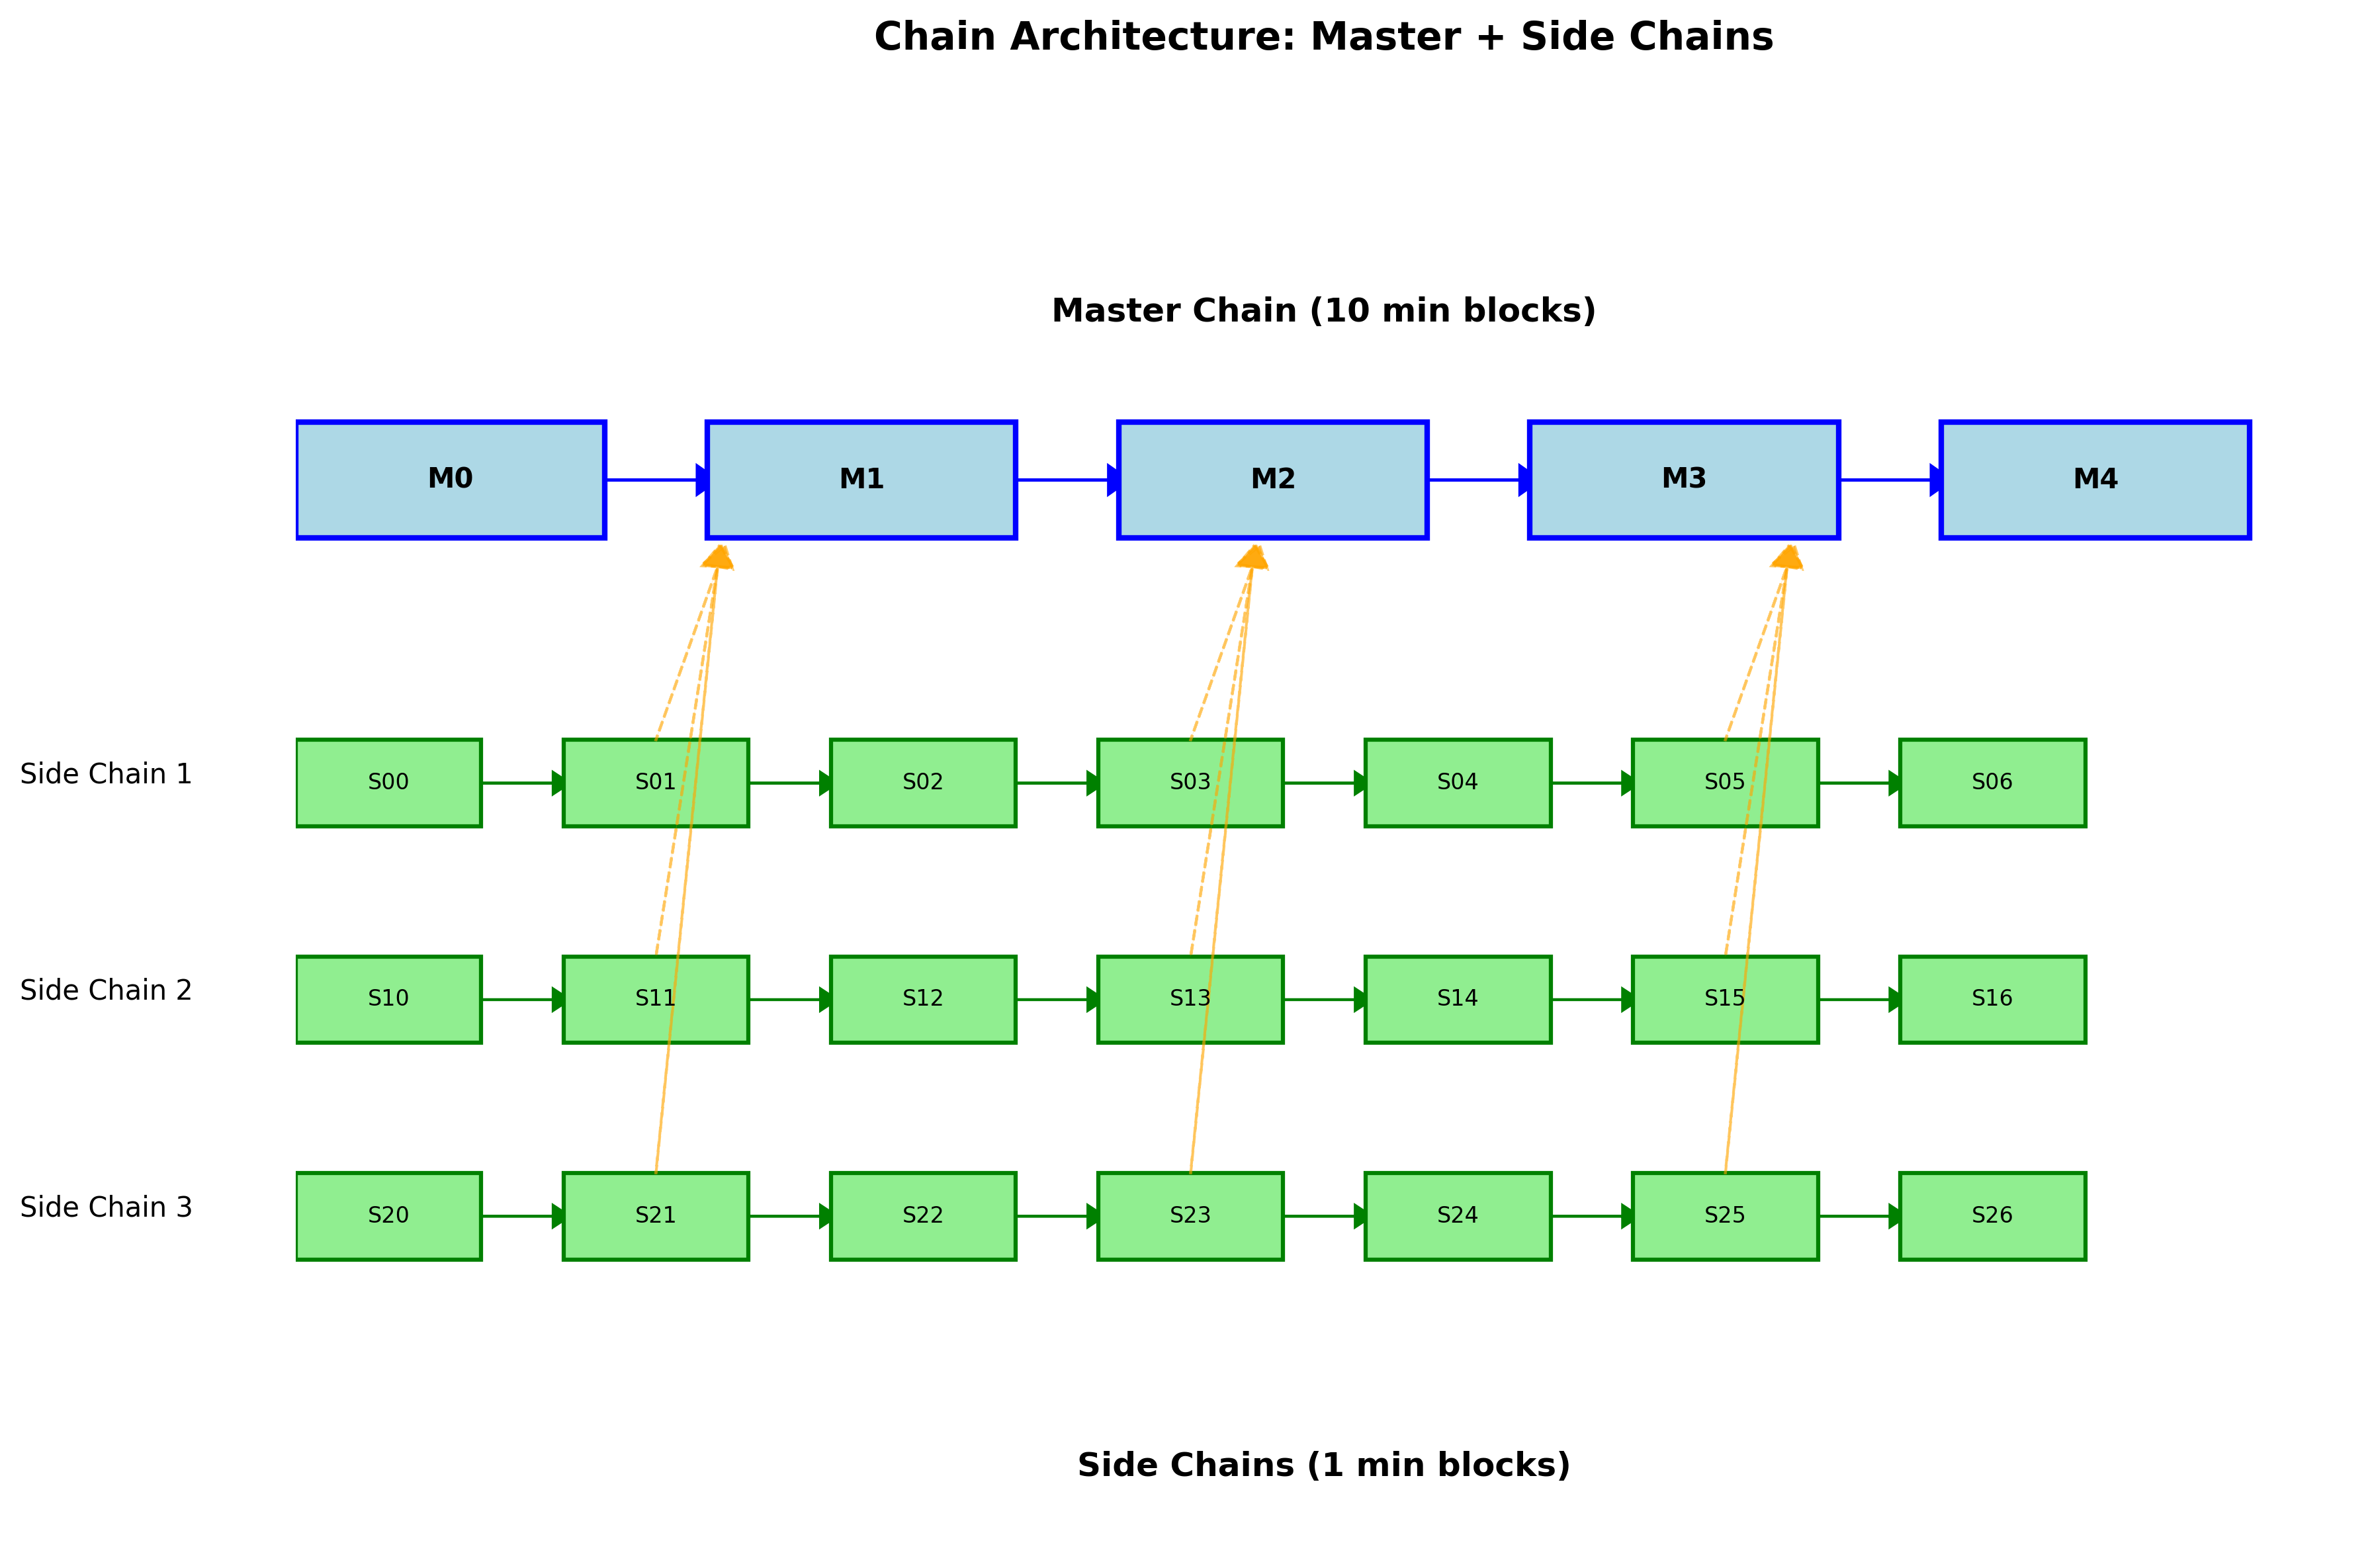
\includegraphics[width=0.9\textwidth]{img/architecture_diagram.png}
\caption{نمای کلی معماری زنجیره اصلی و زنجیره‌های جانبی}
\label{fig:architecture}
\end{figure}

\section{الگوریتم‌های کلیدی}

\subsection{الگوریتم تخصیص تراکنش}

الگوریتم \ref{alg:assign} تخصیص قطعی را پیاده می‌کند و خواص \lr{Validity} و \lr{Agreement} تخصیص را تضمین می‌کند.

\begin{algorithm}[h]
\caption{تخصیص تراکنش به زنجیره جانبی}
\label{alg:assign}
\begin{algorithmic}[1]
\REQUIRE تراکنش $tx$، تعداد زنجیره‌ها $N$
\ENSURE شناسه زنجیره $sid \in \{0,\ldots,N-1\}$
\STATE $u \gets$ اولین \lr{UTXO} ورودی $tx$
\STATE $h \gets \text{SHA256}(u)$ \COMMENT{هش ۲۵۶ بیتی}
\STATE $v \gets$ تبدیل ۸ بایت اول $h$ به عدد صحیح بی‌علامت ۶۴ بیتی
\STATE $sid \gets v \bmod N$
\RETURN $sid$
\end{algorithmic}
\end{algorithm}

پیچیدگی زمانی $O(1)$ است. در پیاده‌سازی Rust: \lr{\texttt{utxo.numeric\_hash() \% num\_side\_chains}}.

\begin{algorithm}[h]
\caption{پردازش و نهایی‌سازی تراکنش}
\label{alg:process}
\begin{algorithmic}[1]
\REQUIRE $tx$، سیستم $\mathcal{S}$
\STATE $sid \gets$ خروجی الگوریتم \ref{alg:assign}
\STATE افزودن $tx$ به $\mathcal{M}_{sid}$
\STATE استخراج بلوک $B_s$ روی $C_{sid}$ (هر $\Delta T_s$)
\STATE ساخت بلوک $B_m$ روی $C_0$ حاوی $\text{Ref}(B_s)$
\IF{$B_m$ دارای $k$ تأیید روی $C_0$}
   \STATE علامت‌گذاری $tx$ به‌عنوان \lr{finalized}
\ENDIF
\end{algorithmic}
\end{algorithm}

\subsection{اجماع و ماژول‌های پیاده‌سازی}

پیاده‌سازی Rust شامل چهار ماژول است: \textbf{رمزنگاری} (\lr{SHA-256}، \lr{ECDSA})، \textbf{اجماع} (انتخاب زنجیره با بیشترین کار، قطعیت پس از $k=6$ تأیید)، \textbf{اعتبارسنجی} (\lr{UTXO set}، جلوگیری از دوبارخرج) و \textbf{تراکنش بین‌زنجیره‌ای} (قفل اتمیک: \lr{Initiated $\rightarrow$ Locked $\rightarrow$ Verified $\rightarrow$ Completed}).

\section{فرآیند پردازش تراکنش}

فرآیند پردازش یک تراکنش مطابق الگوریتم \ref{alg:process} است: ایجاد $tx$ $\rightarrow$ تخصیص به $C_{\mathcal{A}(u)}$ $\rightarrow$ قرارگیری در \lr{mempool} $\rightarrow$ استخراج $B_s$ $\rightarrow$ ارجاع در $B_m$ $\rightarrow$ نهایی‌سازی پس از $k$ تأیید روی $C_0$.

\section{مقایسه مقیاس‌پذیری با روش‌های مشابه}

جدول \ref{tab:scalability-comparison-ch3} معماری پیشنهادی را از نظر \textbf{رشد خطی \lr{TPS}} با راه‌حل‌های مرورشده در فصل دوم مقایسه می‌کند.

\begin{table}[h]
\centering
\caption{مقایسه مقیاس‌پذیری: معماری پیشنهادی در برابر روش‌های مشابه}
\label{tab:scalability-comparison-ch3}
\small
\begin{tabular}{|p{2.8cm}|p{2.2cm}|p{2.4cm}|p{2.6cm}|p{2.4cm}|}
\hline
\textbf{روش} & \textbf{رشد \lr{TPS}} & \textbf{لنگر امنیتی} & \textbf{تغییر \lr{L1}} & \textbf{محدودیت اصلی} \\
\hline
بیتکوین & ثابت ($\sim$7) & خود \lr{L1} & --- & اندازه/فاصله بلوک \\
\hline
لایتنینگ & وابسته به کانال & \lr{L1} (تسویه) & \lr{L2} & نقدینگی، مسیریابی \\
\hline
شاردینگ & خطی با شارد & شارد + \lr{beacon} & زیاد & امنیت/ارتباط بین‌شاردی \\
\hline
زنجیره جانبی (\lr{RSK}) & محدود (یک جانبی) & \lr{merge mining} & پل & تعداد ثابت زنجیره \\
\hline
\textbf{پیشنهادی ($N$ جانبی)} & \textbf{خطی:} $\frac{NS}{\Delta T_s}$ & \textbf{\lr{PoW} $C_0$} & کم & هماهنگی، تراکنش بین‌زنجیره‌ای \\
\hline
\end{tabular}
\end{table}

\textbf{تمایز اصلی:} برخلاف لایتنینگ که مقیاس را به کانال‌های خصوصی واگذار می‌کند، و برخلاف \lr{RSK}/\lr{Liquid} که معمولاً یک یا تعداد محدودی زنجیره دارند، معماری پیشنهادی \textbf{با افزودن $N$، ظرفیت را به‌صورت تقریباً خطی} افزایش می‌دهد (قضیه \ref{thm:linear-scaling}). شاردینگ نیز خطی است اما نیازمند بازطراحی پروتکل و ماشین حالت مشترک است؛ طرح ما بر مدل \lr{UTXO} و \lr{PoW} بیتکوین بنا شده است.

\section{مزایای معماری پیشنهادی}

\subsection{مقیاس‌پذیری افقی}

یکی از مهم‌ترین مزایای این معماری، قابلیت مقیاس‌پذیری افقی است. با افزایش تعداد زنجیره‌های جانبی، ظرفیت کل شبکه به صورت خطی افزایش می‌یابد.

\textbf{نکته بسیار مهم:} با تنها یک زنجیره جانبی، عملکرد سیستم تقریباً مشابه بیتکوین است (فقط با بلوک‌های سریع‌تر). \textbf{مقیاس‌پذیری واقعی از پردازش موازی با چندین زنجیره جانبی حاصل می‌شود}.

\subsubsection{مدل تئوری}

برای محاسبه TPS تئوری از فرمول زیر استفاده می‌شود:

\begin{latin}
\begin{equation}
TPS_{theoretical} = \frac{M}{T_m} + \frac{N \times S}{T_s}
\end{equation}
\end{latin}

که در آن $M$ تعداد تراکنش در هر بلوک زنجیره اصلی، $T_m=600$ ثانیه، $N$ تعداد زنجیره‌های جانبی، $S$ تعداد تراکنش در هر بلوک زنجیره جانبی و $T_s=60$ ثانیه است. با افزایش $N$، TPS کل شبکه به صورت خطی افزایش می‌یابد.

نتایج بنچمارک محاسباتی (ظرفیت \lr{CPU} با دشواری پایین) در جدول \ref{tab:real-benchmark-results} فصل چهارم گزارش شده است. در این فصل بر مدل تئوری و مقایسه با روش‌های مشابه تمرکز می‌کنیم.

زنجیره‌های جانبی هر $\Delta T_s=60$ ثانیه بلوک تولید می‌کنند (در مقایسه با ۱۰ دقیقه در بیتکوین)، لذا تأخیر تأیید اولیه کاهش می‌یابد. امنیت از طریق $C_0$ با \lr{PoW} و دشواری بالا حفظ می‌شود؛ زنجیره‌های جانبی با دشواری پایین‌تر، هزینه استخراج را کاهش می‌دهند در حالی که ارجاع در $C_0$ یکپارچگی را تضمین می‌کند.

\section{محاسبه حداکثر TPS تئوری}

برای تعیین حداکثر ظرفیت تئوری سیستم، محدودیت‌های مختلف باید شناسایی شوند. با فرض اندازه بلوک ۱ مگابایت (مشابه بیتکوین) و میانگین اندازه تراکنش ۲۵۰ بایت:

\begin{latin}
\begin{equation}
\begin{split}
\text{Max\_Tx\_Per\_Block} &= \frac{\text{Block\_Size}}{\text{Avg\_Tx\_Size}} = \frac{1{,}048{,}576}{250} \\
&= 4{,}194
\end{split}
\end{equation}
\end{latin}

با فرض زمان اعتبارسنجی ۱/۰ میلی‌ثانیه برای هر تراکنش:

\begin{latin}
\begin{equation}
\begin{split}
\text{Max\_Tx\_CPU} &= \frac{\text{Block\_Time}}{\text{Validation\_Time}} = \frac{60{,}000\ \text{ms}}{0.1\ \text{ms}} \\
&= 600{,}000
\end{split}
\end{equation}
\end{latin}

و با فرض زمان تایید امضای دیجیتال ۵/۰ میلی‌ثانیه:

\begin{latin}
\begin{equation}
\text{Max\_Tx\_Crypto} = \frac{60{,}000\ \text{ms}}{0.5\ \text{ms}} = 120{,}000
\end{equation}
\end{latin}

گلوگاه \lr{(Bottleneck)} سیستم، کوچک‌ترین محدودیت است:

\begin{latin}
\begin{equation}
\begin{split}
\text{Bottleneck} &= \min(4{,}194,\ 600{,}000,\ 120{,}000,\ \ldots) \\
&= 4{,}194
\end{split}
\end{equation}
\end{latin}

بنابراین اندازه بلوک محدودیت اصلی سیستم است. با استفاده از این محدودیت، TPS کل سیستم به صورت زیر محاسبه می‌شود:

\begin{latin}
\begin{equation}
TPS_{total} = \frac{M}{T_m} + \frac{N \times S}{T_s}
\end{equation}
\end{latin}

که در آن $M=S=4{,}194$، $T_m=600$ و $T_s=60$ ثانیه و $N$ تعداد زنجیره‌های جانبی است. با جایگذاری مقادیر:

\begin{latin}
\begin{align}
TPS_{master} &= \frac{4,194}{600} = 6.99 \\
TPS_{side} &= \frac{N \times 4,194}{60} = 69.90 \times N \\
TPS_{total} &= 6.99 + (69.90 \times N)
\end{align}
\end{latin}

\begin{table}[h]
\centering
\caption{مقیاس‌پذیری شبکه: TPS تئوری برای 1 تا 1000 زنجیره جانبی}
\label{tab:theoretical-max-tps}
\begin{tabular}{|c|c|c|c|c|}
\hline
\textbf{زنجیره‌های جانبی} & \textbf{TPS زنجیره اصلی} & \textbf{TPS زنجیره‌های جانبی} & \textbf{TPS کل} & \textbf{بهبود نسبت به بیتکوین} \\ \hline
\textbf{1} & 6.99 & 69.90 & \textbf{76.89} & \textbf{11.0x} \\ \hline
3 & 6.99 & 209.70 & 216.69 & 30.96x \\ \hline
5 & 6.99 & 349.50 & 356.49 & 50.93x \\ \hline
10 & 6.99 & 699.00 & 705.99 & 100.86x \\ \hline
20 & 6.99 & 1,398.00 & 1,404.99 & 200.71x \\ \hline
50 & 6.99 & 3,495.00 & 3,501.99 & 500.28x \\ \hline
\textbf{100} & 6.99 & 6,990.00 & \textbf{6,996.99} & \textbf{999.57x} \\ \hline
\textbf{1000} & 6.99 & 69,900.00 & \textbf{69,906.99} & \textbf{9,986.7x} \\ \hline
\end{tabular}
\end{table}

با تنها ۱ زنجیره جانبی، TPS تنها ۱۱ برابر بیتکوین است (۷۶/۸۹ TPS) و بدون پردازش موازی بهبود محدود است. با افزودن هر زنجیره جانبی، دقیقاً ۶۹/۹۰ TPS به ظرفیت کل اضافه می‌شود و رابطه کاملاً خطی است:
    \begin{latin}
    \begin{equation}
    \frac{\Delta TPS}{\Delta N} = 69.90 \text{ TPS per side chain}
    \end{equation}
    \end{latin}
برای کاربردهای تجاری، ۱۰ تا ۱۰۰ زنجیره جانبی می‌تواند ۷۰۶ تا ۶٬۹۹۷ TPS فراهم کند. با ۱۰۰۰ زنجیره جانبی، سیستم قادر به پردازش ۶۹٬۹۰۷ TPS است که تقریباً ۱۰٬۰۰۰ برابر بیتکوین است. معماری پیشنهادی محدودیت نظری برای تعداد زنجیره‌های جانبی ندارد و تنها محدودیت، منابع سخت‌افزاری و شبکه است.

\begin{table}[h]
\centering
\caption{مقایسه عملکرد واقعی با حداکثر تئوری}
\label{tab:actual-vs-theoretical}
\begin{tabular}{|c|c|c|c|}
\hline
\textbf{متریک} & \textbf{مقدار \lr{(TPS)}} & \textbf{بهبود \lr{vs} بیتکوین} & \textbf{محدودیت} \\ \hline
\multicolumn{4}{|c|}{\textbf{عملکرد واقعی (بنچمارک Rust با دشواری پایین)}} \\ \hline
ظرفیت محاسباتی (1 زنجیره) & 44,824.87 & 6,403x & CPU/Memory \\ \hline
میانگین عملکرد واقعی & 16,433.95 & 2,347x & Coordination \\ \hline
\multicolumn{4}{|c|}{\textbf{TPS تئوری شبکه (با محدودیت‌های واقعی 1MB block)}} \\ \hline
شبکه واقعی (1 زنجیره) & 76.89 & 11x & اندازه بلوک \\ \hline
شبکه واقعی (10 زنجیره) & 705.99 & 101x & اندازه بلوک \\ \hline
شبکه واقعی (100 زنجیره) & 6,996.99 & 1,000x & اندازه بلوک \\ \hline
شبکه واقعی (1000 زنجیره) & 69,906.99 & 10,000x & اندازه بلوک \\ \hline
\end{tabular}
\end{table}

عدد ۴۴٬۸۲۴ TPS از بنچمارک با دشواری PoW پایین به دست آمده و سرعت خالص پردازش Rust در شرایط ایده‌آل را نشان می‌دهد. در شبکه واقعی با محدودیت بلوک ۱MB و دشواری بالای بیتکوین، TPS بین ۷۷ تا ۷۰٬۰۰۰ است که اعداد واقع‌بینانه‌تری هستند. مقیاس‌پذیری واقعی از پردازش موازی حاصل می‌شود: با ۱ زنجیره جانبی فقط ۱۱ برابر بهتر از بیتکوین، با ۱۰ زنجیره ۱۰۱ برابر، با ۱۰۰ زنجیره ۱٬۰۰۰ برابر و با ۱۰۰۰ زنجیره ۱۰٬۰۰۰ برابر بهبود داریم. در شبکه واقعی، اندازه بلوک (۱MB) گلوگاه اصلی است و سیستم ظرفیت محاسباتی ۵۸۳ برابر بیشتر از این محدودیت دارد. هر زنجیره جانبی دقیقاً ۶۹/۹ TPS اضافه می‌کند و با افزایش اندازه بلوک به ۴MB یا استفاده از SegWit می‌توان TPS را ۴ برابر کرد. با سرور پیشرفته (۶۴ هسته، ۱ Gbps) حدود ۴۲٬۰۰۰ TPS، با کلاستر توزیع‌شده ۱۰ نود بیش از ۴۰۰٬۰۰۰ TPS و با افزایش اندازه بلوک به ۴MB حدود ۲۸٬۰۰۰ TPS با ۱۰۰ زنجیره جانبی قابل دستیابی است.

\section{چرا یک زنجیره جانبی کافی نیست؟}

صرفاً داشتن یک زنجیره با بلوک‌های سریع‌تر، مقیاس‌پذیری \textbf{خطی} ایجاد نمی‌کند. این ادعا را به‌صورت رسمی بیان می‌کنیم.

\begin{theorem}[کران بالای تک‌زنجیره سریع]
\label{thm:single-chain-bound}
فرض کنید اندازه بلوک $B$، میانگین اندازه تراکنش $\tau$ و فاصله بلوک جانبی $\Delta T_s$ ثابت باشد. با یک زنجیره جانبی ($N=1$):
\begin{latin}
\[
TPS_{total} \leq \frac{M}{\Delta T_m} + \frac{\lfloor B/\tau \rfloor}{\Delta T_s}
\]
\end{latin}
برای $B=1$MB، $\tau=250$ بایت، $\Delta T_m=600$s، $\Delta T_s=60$s: $TPS_{total} \leq 6.99 + 69.90 = 76.89$ که حدود $11\times$ بیتکوین است.
\end{theorem}

\begin{proof}[ایده اثبات]
سهم زنجیره اصلی از $M/\Delta T_m$ محدود است. سهم جانبی از ظرفیت یک بلوک در هر $\Delta T_s$ بیشتر نمی‌شود. کاهش $\Delta T_s$ بدون افزایش $N$ فقط همان سهم را تقسیم می‌کند و با محدودیت $B$ به سقف $\lfloor B/\tau \rfloor/\Delta T_s$ می‌رسد. کاهش بیش از حد دشواری \lr{PoW} امنیت را تضعیف می‌کند (محدودیت عملی دیگر).
\end{proof}

\begin{theorem}[مقیاس‌پذیری خطی با $N$ زنجیره]
\label{thm:linear-scaling}
با فرض $S_i=S$ برای همه $i$ و ثابت بودن $\Delta T_m,\Delta T_s$:
\begin{latin}
\[
TPS_{total}(N) = \frac{M}{\Delta T_m} + \frac{N \cdot S}{\Delta T_s}, \qquad
\frac{\partial TPS_{total}}{\partial N} = \frac{S}{\Delta T_s} > 0
\]
\end{latin}
بنابراین هر زنجیره جانبی جدید، به‌صورت خطی ظرفیت اضافه می‌کند.
\end{theorem}

\begin{proof}[ایده اثبات]
جمع مستقل ظرفیت $N$ زنجیره موازی است؛ زنجیره اصلی بار تراکنش کامل را تکرار نمی‌کند و فقط ارجاع ثبت می‌کند. در مدل تئوری، $M$ ثابت و سهم جانبی با $N$ رشد می‌کند.
\end{proof}

با $N=10$، $100$، $1000$ به ترتیب حدود $706$، $6997$ و $69907$ \lr{TPS} تئوری (با پارامترهای جدول \ref{tab:theoretical-max-tps}) حاصل می‌شود. هر زنجیره جانبی مستقل کار می‌کند و $C_0$ فقط ارجاعات را نگه می‌دارد.

\begin{figure}[h]
\centering
\begin{latin}
\begin{equation}
\begin{split}
TPS_{\text{total}} &= TPS_{\text{master}} + \sum_{i=1}^{N} TPS_{\text{side}_{i}} \\
&= 6.99 + N \times 69.90
\end{split}
\end{equation}
\end{latin}
\caption{فرمول مقیاس‌پذیری افقی: TPS به صورت خطی با تعداد زنجیره‌ها رشد می‌کند}
\label{fig:scaling-formula}
\end{figure}

\subsection{مقایسه رویکردها}

\begin{table}[h]
\centering
\caption{مقایسه رویکرد تک زنجیره \lr{vs} چند زنجیره}
\label{tab:single-vs-multi-chain}
\begin{tabular}{|p{4cm}|p{5cm}|p{5cm}|}
\hline
\textbf{ویژگی} & \textbf{یک زنجیره سریع} & \textbf{چندین زنجیره موازی} \\ \hline
حداکثر TPS ممکن & محدود (< 100 TPS) & نامحدود (خطی با N) \\ \hline
امنیت & کاهش با بلوک‌های خیلی سریع & حفظ شده با PoW \\ \hline
پیچیدگی & کم & متوسط \\ \hline
مقیاس‌پذیری & محدود & عالی \\ \hline
نیاز به سخت‌افزار & بالا (یک نود قدرتمند) & توزیع شده \\ \hline
\end{tabular}
\end{table}

معماری پیشنهادی از دو استراتژی استفاده می‌کند: بلوک‌های سریع‌تر در زنجیره‌های جانبی (۱۰ دقیقه به ۱ دقیقه) که ۱۰ برابر بهبود می‌دهد، و پردازش موازی با N زنجیره که N برابر بهبود ایجاد می‌کند؛ ترکیب آن‌ها در مجموع $10 \times N$ برابر بهبود نسبت به بیتکوین می‌دهد. یکی از چالش‌های اصلی، تراکنش‌هایی است که UTXOهای زنجیره‌های مختلف را شامل می‌شوند؛ راه‌حل‌ها شامل استفاده از تراکنش‌های دو مرحله‌ای، پروتکل قفل اتمیک و تایید متقابل بین زنجیره‌هاست. با دشواری پایین‌تر زنجیره‌های جانبی، امکان حمله ۵۱٪ وجود دارد که با الگوریتم تخصیص ماینر برای مشارکت هر ماینر در چند زنجیره، چک‌پوینت‌های دوره‌ای در زنجیره اصلی و مکانیزم تشخیص و بازگشت تراکنش‌های مخرب می‌توان آن را کاهش داد. پیاده‌سازی این معماری پیچیده‌تر از بلاکچین ساده است و برای کاهش پیچیدگی، استفاده از معماری ماژولار، جداسازی منطق زنجیره اصلی و جانبی و ایجاد APIهای استاندارد پیشنهاد می‌شود.

\section{جمع‌بندی}

در این فصل، معماری سیستم بلاکچین پیشنهادی را به تفصیل تشریح کردیم. این معماری با استفاده از ساختار زنجیره اصلی و زنجیره‌های جانبی، قادر به افزایش قابل توجه TPS نسبت به بلاکچین بیتکوین است، در حالی که امنیت و غیرمتمرکز بودن شبکه را حفظ می‌کند. در فصل بعد، به نتایج آزمایشات و مقایسه عملکرد این سیستم با بیتکوین خواهیم پرداخت.


		% فصل سوم: معماری سیستم بلاکچین پیشنهادی
% !TeX root=main.tex
\chapter{نتایج آزمایشات و ارزیابی عملکرد}
\section{مقدمه}

هدف این فصل ارزیابی معماری پیشنهادی از دو دیدگاه است: نخست، مدل نظری ظرفیت که بر اساس اندازه بلوک، فاصله بلوک و تعداد زنجیره‌های جانبی محاسبه می‌شود؛ دوم، بنچمارک\LTRfootnote{Benchmark} پیاده‌سازی به زبان راست\LTRfootnote{Rust} که ظرفیت محاسباتی نمونه اولیه را در محیط آزمایش نشان می‌دهد. تفکیک این دو دیدگاه ضروری است. عددی که در بنچمارک محاسباتی با دشواری پایین و بدون محدودیت واقعی شبکه به دست می‌آید، معادل توان عملیاتی یک شبکه عمومی واقعی نیست؛ بلکه نشان‌دهنده سقف پردازشی نرم‌افزار تحت شرایط کنترل‌شده است.

\section{محیط آزمایش}

پیاده‌سازی نمونه اولیه با زبان راست و در حالت انتشار بهینه‌شده\LTRfootnote{Release Mode} اجرا شده است. معیار اصلی اندازه‌گیری، زمان واقعی اجرا\LTRfootnote{Wall-clock Time} برای پردازش تعداد مشخصی تراکنش در پیکربندی‌های مختلف است. در نسخه فعلی، شبکه همتا‌به‌همتای کامل، تأخیر انتشار بلوک در اینترنت، رفتار خصمانه\LTRfootnote{Adversarial}، تأخیر جغرافیایی، و هزینه واقعی اعتبارسنجی امضا در مقیاس شبکه عمومی به طور کامل مدل نشده‌اند. بنابراین، نتایج آزمایش باید به عنوان ارزیابی نمونه اولیه و نه بنچمارک نهایی تولیدی تفسیر شود.

\begin{table}[h]
\centering
\caption{جدول ۴-۱. پارامترهای آزمایش}
\small
\begin{tabular}{|p{5.5cm}|p{8cm}|}
\hline
پارامتر & مقدار/توضیح \\
\hline
زبان پیاده‌سازی & راست \\
\hline
حالت اجرا & انتشار / بهینه‌شده \\
\hline
ساختار سیستم & زنجیره اصلی + \(N\) زنجیره جانبی \\
\hline
تعداد زنجیره‌های جانبی آزمایشی & ۱، ۲، ۳، ۵، ۱۰ \\
\hline
دشواری اثبات کار در آزمایش & پایین، برای اندازه‌گیری ظرفیت محاسباتی \\
\hline
معیار اصلی & تراکنش بر ثانیه، میانگین، میانه، حداقل، حداکثر، انحراف معیار \\
\hline
محدودیت شبکه واقعی & در این بنچمارک کامل اعمال نشده است \\
\hline
\end{tabular}
\end{table}

\section{مدل نظری شبکه}

با فرض بلوک یک مگابایتی و اندازه متوسط تراکنش ۲۵۰ بایت، تعداد تراکنش در هر بلوک حدود ۴۱۹۴ خواهد بود. اگر زنجیره اصلی هر ۶۰۰ ثانیه و زنجیره جانبی هر ۶۰ ثانیه بلوک تولید کند، داریم:

\begin{latin}
\[
TPS_{total} = 6.99 + 69.90N
\]
\end{latin}

\begin{figure}[h]
\centering
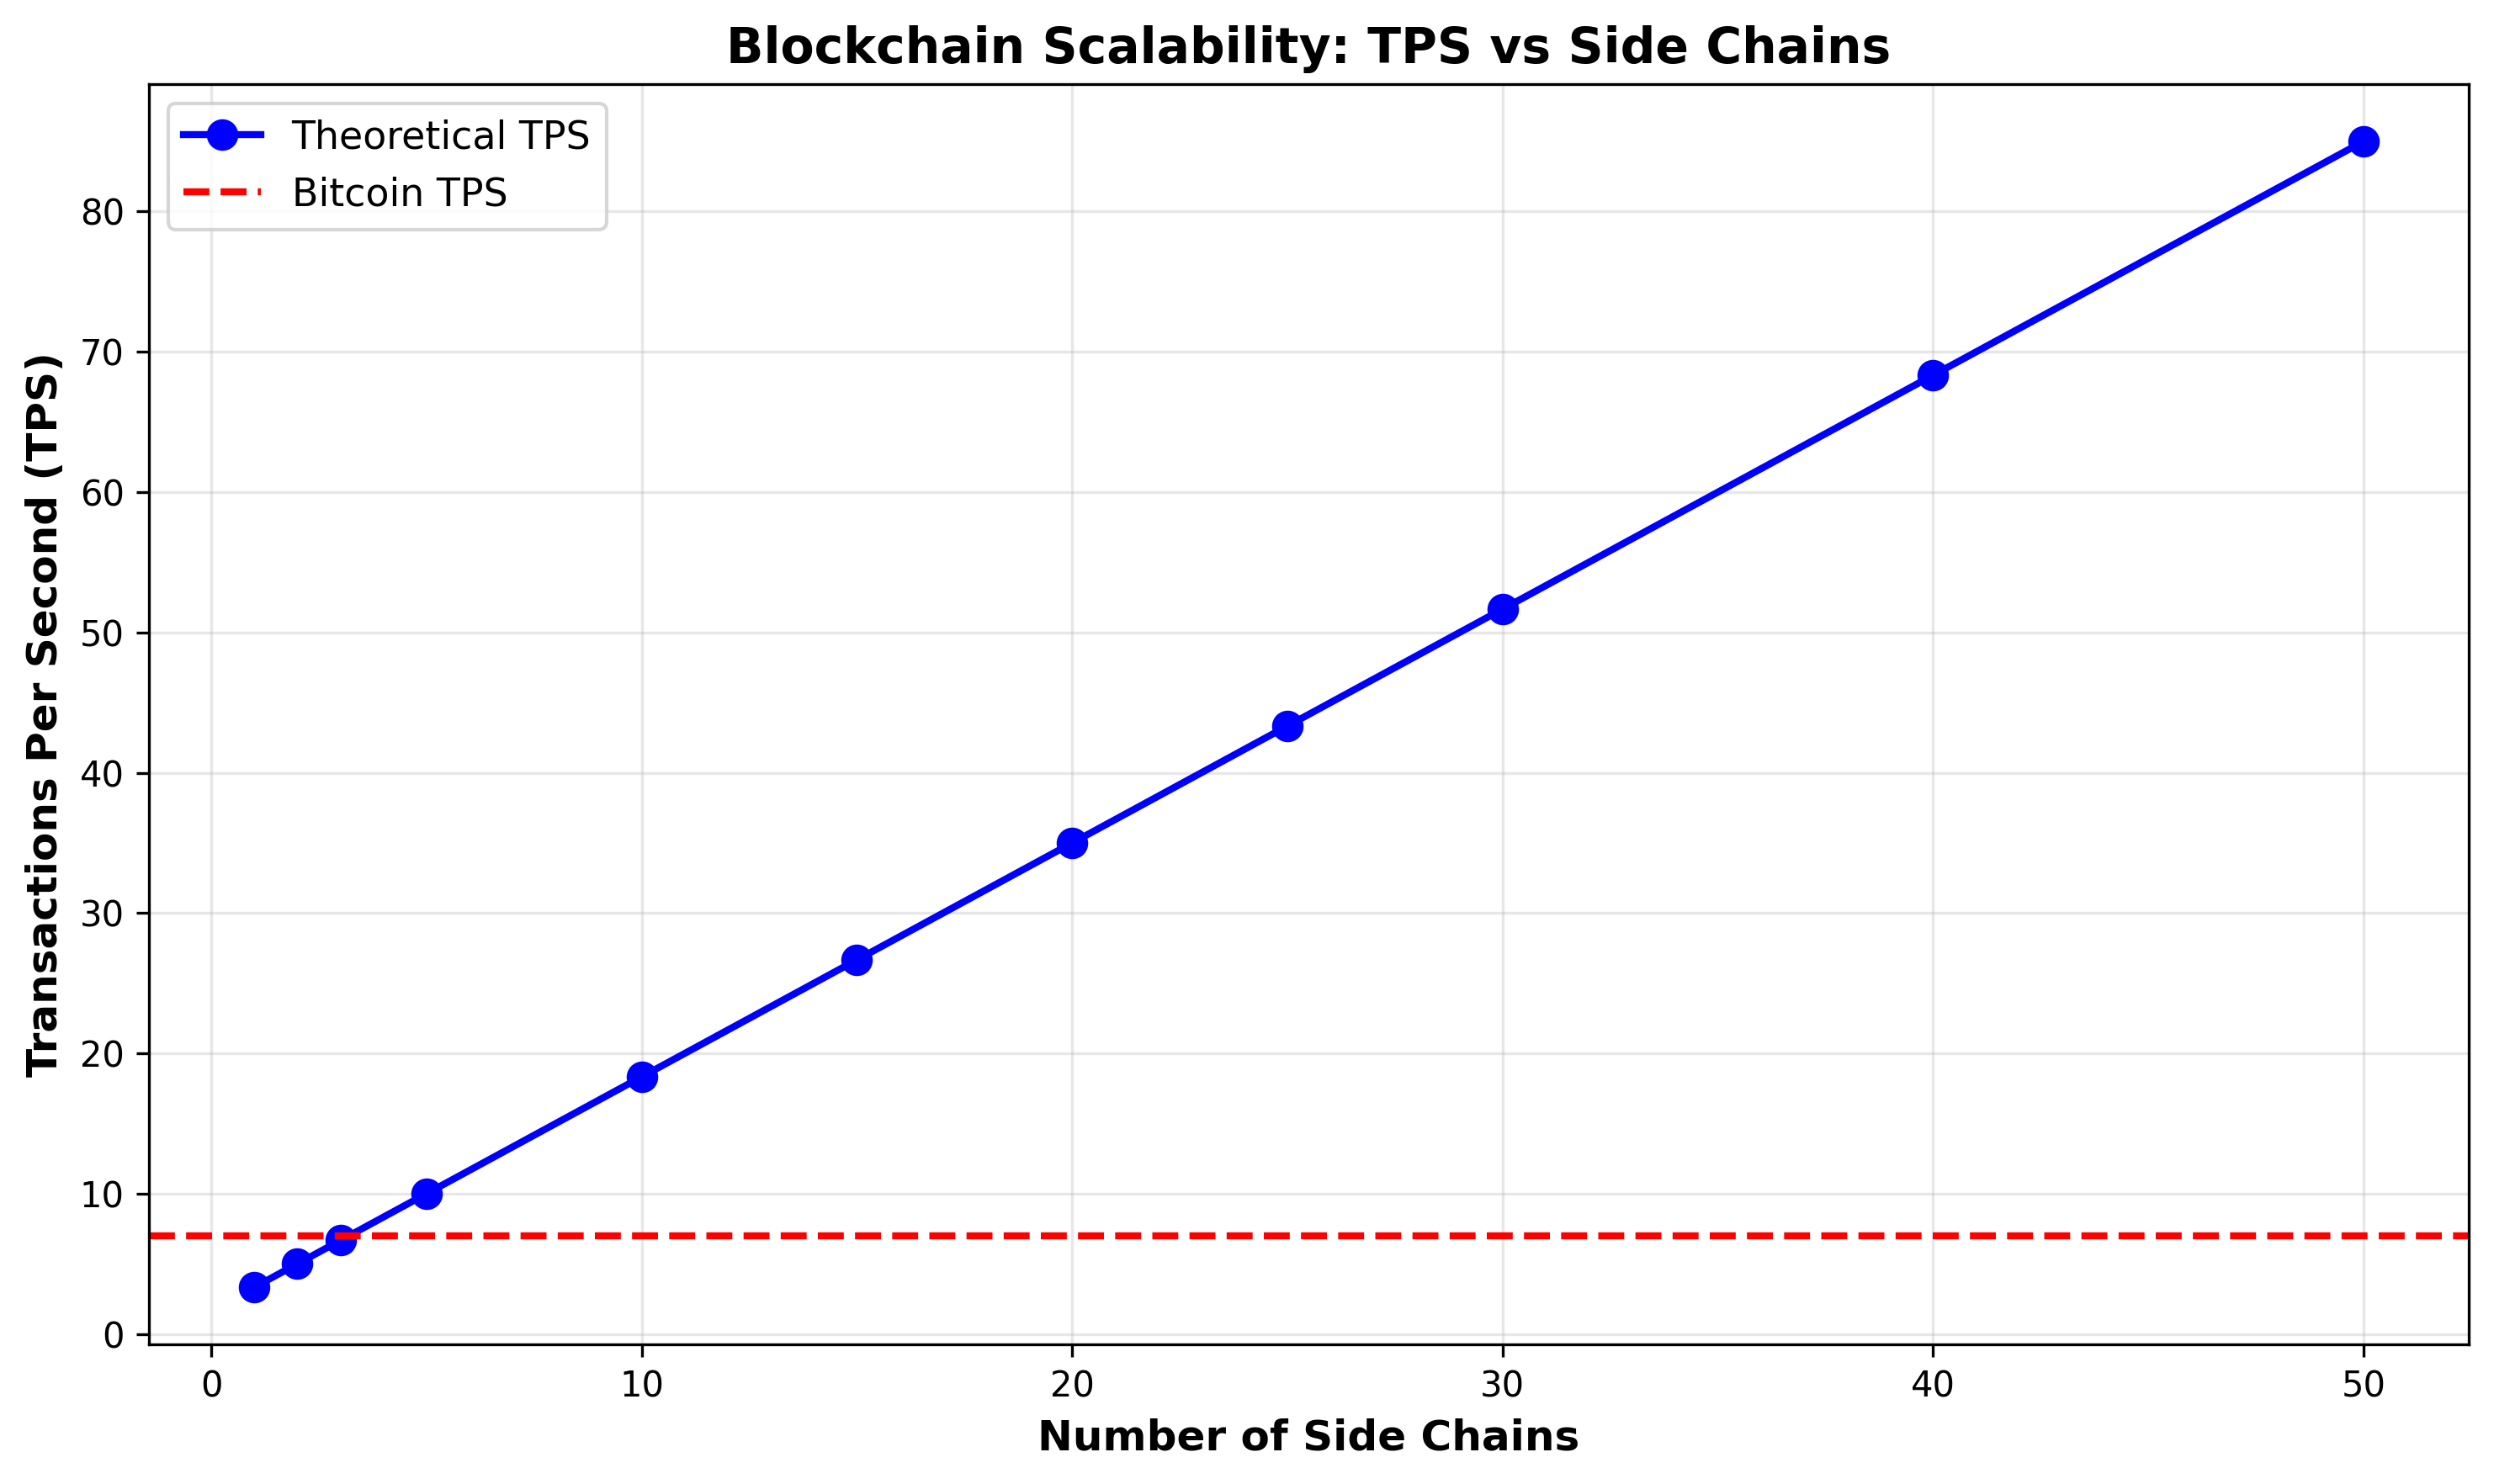
\includegraphics[width=0.92\linewidth]{img/tps_vs_sidechains.png}
\caption{مدل رشد خطی توان عملیاتی با تعداد زنجیره‌های جانبی}
\label{fig:tps-scalability}
\end{figure}


\begin{table}[h]
\centering
\caption{جدول ۴-۲. توان عملیاتی نظری با فرض بلوک یک مگابایتی و تراکنش ۲۵۰ بایتی}
\small
\begin{tabular}{|p{2.2cm}|p{2.8cm}|p{2.5cm}|p{2.8cm}|p{2.8cm}|}
\hline
تعداد زنجیره جانبی & توان زنجیره اصلی & توان زنجیره‌های جانبی & توان کل & بهبود نسبت به ۷ تراکنش بر ثانیه \\
\hline
۱ & ۶.۹۹ & ۶۹.۹۰ & ۷۶.۸۹ & ۱۱.۰ برابر \\
\hline
۳ & ۶.۹۹ & ۲۰۹.۷۰ & ۲۱۶.۶۹ & ۳۱.۰ برابر \\
\hline
۵ & ۶.۹۹ & ۳۴۹.۵۰ & ۳۵۶.۴۹ & ۵۰.۹ برابر \\
\hline
۱۰ & ۶.۹۹ & ۶۹۹.۰۰ & ۷۰۵.۹۹ & ۱۰۰.۹ برابر \\
\hline
۲۰ & ۶.۹۹ & ۱۳۹۸.۰۰ & ۱۴۰۴.۹۹ & ۲۰۰.۷ برابر \\
\hline
۵۰ & ۶.۹۹ & ۳۴۹۵.۰۰ & ۳۵۰۱.۹۹ & ۵۰۰.۳ برابر \\
\hline
۱۰۰ & ۶.۹۹ & ۶۹۹۰.۰۰ & ۶۹۹۶.۹۹ & ۹۹۹.۶ برابر \\
\hline
\end{tabular}
\end{table}

این جدول نشان می‌دهد که بهبود اصلی از تعداد زنجیره‌های جانبی می‌آید، نه صرفاً کوتاه‌تر کردن زمان بلوک. با یک زنجیره جانبی، ظرفیت حدود ۷۷ تراکنش بر ثانیه\LTRfootnote{Transactions Per Second (TPS)} است؛ با ۱۰۰ زنجیره جانبی، ظرفیت نظری به حدود ۷۰۰۰ تراکنش بر ثانیه می‌رسد.

\section{نتایج بنچمارک پیاده‌سازی}

نتایج بنچمارک نمونه اولیه در جدول زیر گزارش شده است.

\begin{table}[h]
\centering
\caption{جدول ۴-۳. نتایج بنچمارک محاسباتی پیاده‌سازی به زبان راست}
\small
\begin{tabular}{|p{1.4cm}|p{1.5cm}|p{1.5cm}|p{1.5cm}|p{1.5cm}|p{1.5cm}|p{1.6cm}|}
\hline
تعداد زنجیره جانبی & تعداد تراکنش آزمون & میانگین توان & میانه توان & حداقل توان & حداکثر توان & انحراف معیار \\
\hline
۱ & ۵۰ & ۴۴٬۸۲۴.۸۷ & ۴۵٬۰۶۸.۷۲ & ۳۹٬۲۳۲.۳۳ & ۵۰٬۱۷۳.۵۵ & ۵٬۴۷۴.۶۸ \\
\hline
۲ & ۱۰۰ & ۷٬۶۱۹.۸۹ & ۴٬۸۹۰.۹۹ & ۳٬۳۱۴.۷۱ & ۱۴٬۶۵۳.۹۸ & ۶٬۱۴۲.۴۷ \\
\hline
۳ & ۱۵۰ & ۷٬۰۴۹.۸۴ & ۷٬۱۱۳.۳۰ & ۵٬۰۸۵.۸۵ & ۸٬۹۵۰.۳۷ & ۱٬۹۳۳.۰۴ \\
\hline
۵ & ۲۵۰ & ۱۳٬۷۴۰.۷۰ & ۱۳٬۶۹۰.۸۸ & ۹٬۶۶۳.۱۱ & ۱۷٬۸۶۸.۱۰ & ۴٬۱۰۲.۷۲ \\
\hline
۱۰ & ۵۰۰ & ۸٬۹۳۴.۴۶ & ۱۰٬۱۱۷.۴۵ & ۶٬۱۴۴.۶۰ & ۱۰٬۵۴۱.۳۴ & ۲٬۴۲۵.۳۷ \\
\hline
\end{tabular}
\end{table}

این اعداد ظرفیت محاسباتی نمونه اولیه را نشان می‌دهند. مقدار بسیار بالای توان عملیاتی در حالت یک زنجیره جانبی به این دلیل است که محدودیت واقعی تولید بلوک، انتشار شبکه، اندازه بلوک و دشواری واقعی اثبات کار اعمال نشده است. همچنین، کاهش توان در برخی پیکربندی‌های چندزنجیره‌ای نشان می‌دهد سربار هماهنگی، مدیریت ساختارهای داده، تعویض زمینه پردازشی\LTRfootnote{Context Switching} و همزمانی می‌تواند اثر قابل توجهی داشته باشد.

\section{تحلیل تفاوت مدل نظری و بنچمارک}

وجود اختلاف میان مدل نظری شبکه و بنچمارک محاسباتی طبیعی است. مدل نظری بر محدودیت اندازه بلوک و فاصله بلوک مبتنی است. بنچمارک محاسباتی، زمان پردازش داخلی برنامه را اندازه می‌گیرد. بنابراین، اگر یک اجرای آزمایشی بتواند ده‌ها هزار تراکنش بر ثانیه پردازش کند، به این معنی نیست که شبکه عمومی با همان عدد نهایی می‌شود. شبکه واقعی با محدودیت‌های زیر روبه‌روست:

\begin{itemize}
\item انتشار بلوک میان نودهای جغرافیایی مختلف.
\item تأخیر شبکه و اتلاف بسته\LTRfootnote{Packet Loss}.
\item اعتبارسنجی امضاها و اسکریپت‌ها.
\item محدودیت اندازه بلوک و سیاست استخر تراکنش\LTRfootnote{Mempool}.
\item رقابت ماینرها و احتمال فورک\LTRfootnote{Fork}.
\item داده‌دسترسی بلوک‌های جانبی.
\item رفتار مهاجم و حملات منع سرویس\LTRfootnote{Denial of Service (DoS)}.
\end{itemize}

به همین دلیل، در سراسر این پایان‌نامه عددهایی مانند ۴۴٬۸۲۴ تراکنش بر ثانیه، «ظرفیت محاسباتی پیاده‌سازی در محیط کنترل‌شده» نامیده می‌شوند و نه توان عملیاتی شبکه واقعی؛ این دو کمیت از جنس متفاوتی هستند و خلط آن‌ها رایج‌ترین خطای گزارش‌دهی در کارهای مشابه است.

\section{مقایسه با راهکارهای موجود}

\begin{table}[h]
\centering
\caption{جدول ۴-۴. مقایسه کیفی معماری پیشنهادی با راهکارهای مقیاس‌پذیری}
\small
\begin{tabular}{|p{1.8cm}|p{1.6cm}|p{1.6cm}|p{1.6cm}|p{1.6cm}|p{1.8cm}|}
\hline
راهکار & مکانیزم & امنیت & پیچیدگی کاربر & رشد ظرفیت & محدودیت اصلی \\
\hline
بیتکوین پایه & لایه اول تک‌زنجیره‌ای & بسیار بالا & کم & ثابت & اندازه و زمان بلوک \\
\hline
افزایش اندازه بلوک & لایه اول بزرگ‌تر & بالا، با هزینه نود & کم & محدود & تمرکز نود \\
\hline
لایتنینگ & کانال پرداخت & وابسته به لایه اول و کانال & متوسط/بالا & وابسته به نقدینگی & مسیریابی و نقدینگی \\
\hline
رول‌آپ & اجرای برون‌زنجیره‌ای + اثبات/داده & نزدیک به لایه اول & متوسط & بالا & داده‌دسترسی و مرتب‌ساز \\
\hline
شاردینگ & تقسیم حالت/تراکنش & وابسته به شارد & پنهان از کاربر & خطی & امنیت شارد و تراکنش بین‌شاردی \\
\hline
زنجیره جانبی کلاسیک & زنجیره مستقل & وابسته به پل/اجماع & متوسط & متغیر & مدل اعتماد \\
\hline
معماری پیشنهادی & چند زنجیره جانبی + زنجیره اصلی & امنیت نهایی از زنجیره اصلی & متوسط & تقریباً خطی با \(N\) & تراکنش بین‌زنجیره‌ای و هماهنگی \\
\hline
\end{tabular}
\end{table}

\section{تحلیل حساسیت}

برای تحلیل حساسیت، می‌توان اثر سه پارامتر اصلی را بررسی کرد: تعداد زنجیره‌های جانبی، اندازه بلوک و فاصله بلوک جانبی. طبق مدل:

\begin{latin}
\[
TPS = \frac{M}{T_m} + \frac{NS}{T_s}
\]
\end{latin}

افزایش \(N\) اثر خطی دارد. افزایش \(S\)، که معمولاً تابع اندازه بلوک است، نیز اثر خطی دارد، اما هزینه نود را افزایش می‌دهد. کاهش \(T_s\) ظرفیت را افزایش می‌دهد، اما احتمال فورک و فشار انتشار را بالا می‌برد. بنابراین، انتخاب پارامترها باید با توجه به هدف سامانه انجام شود. برای یک شبکه عمومی، محافظه‌کاری در \(T_s\) و \(S\) ضروری است؛ اما در یک شبکه سازمانی یا مجوزدار\LTRfootnote{Permissioned}، می‌توان پارامترها را تهاجمی‌تر انتخاب کرد.

\section{تهدیدهای اعتبار ارزیابی}

اعتبار نتایج این پایان‌نامه از چند جهت محدود است:

\begin{itemize}
\item \textbf{اعتبار داخلی:} ممکن است اندازه نمونه تراکنش‌ها، دشواری پایین یا ساختار داده‌های ساده باعث افزایش مصنوعی توان اندازه‌گیری‌شده شده باشد.
\item \textbf{اعتبار خارجی:} نتایج روی یک محیط آزمایشی الزاماً به شبکه جهانی با هزاران نود تعمیم‌پذیر نیست.
\item \textbf{اعتبار سازه‌ای:} توان عملیاتی به تنهایی معیار کامل نیست و باید تأخیر، قطعیت نهایی، نرخ فورک و هزینه نود نیز بررسی شود.
\item \textbf{اعتبار بازتولید:} برای بازتولید، باید نسخه کد، سخت‌افزار، سیستم‌عامل، پارامترها و روش اجرای بنچمارک ثبت شود.
\end{itemize}

\section{پیشنهاد پروتکل ارزیابی کامل‌تر}

برای ارزیابی دقیق‌تر در آینده، پیشنهاد می‌شود آزمایش‌ها در چهار سطح انجام شوند:

\begin{enumerate}
\item \textbf{آزمایش واحد:} اعتبارسنجی تراکنش، خروجی‌های خرج‌نشده، هش و امضا.
\item \textbf{آزمایش محلی:} اجرای چند زنجیره روی یک ماشین برای سنجش سربار نرم‌افزاری.
\item \textbf{آزمایش شبکه کنترل‌شده:} اجرای نودها روی چند ماشین یا کانتینر با تأخیر مصنوعی.
\item \textbf{آزمایش خصمانه:} شبیه‌سازی حملات دوبارخرج، تأخیر انتشار، فورک و سانسور.
\end{enumerate}

همچنین بهتر است برای هر پیکربندی حداقل ۳۰ تکرار انجام شود و علاوه بر میانگین، فاصله اطمینان و نمودار توزیع گزارش گردد.

\section{تحلیل حذف اجزا}

برای اینکه سهم هر جزء معماری روشن شود، انجام مطالعه حذف اجزا\LTRfootnote{Ablation Study} ضروری است. در این نوع مطالعه، هر بار یکی از اجزای معماری حذف یا ساده‌سازی می‌شود و اثر آن بر عملکرد و امنیت اندازه‌گیری می‌گردد. برای این پایان‌نامه، چند آزمایش حذف مهم پیشنهاد می‌شود:

\begin{itemize}
\item اجرای سیستم با یک زنجیره جانبی در برابر چند زنجیره جانبی، برای سنجش اثر موازی‌سازی.
\item حذف ثبت ارجاع در زنجیره اصلی، برای نشان دادن نقش لنگر امنیتی.
\item اجرای تابع تخصیص تصادفی در برابر تابع تخصیص مبتنی بر خروجی‌های خرج‌نشده، برای سنجش اثر سازگاری و دوبارخرج.
\item افزایش تدریجی دشواری اثبات کار جانبی، برای بررسی رابطه امنیت و توان عملیاتی.
\item فعال و غیرفعال کردن تراکنش بین‌زنجیره‌ای، برای سنجش سربار بین‌زنجیره‌ای.
\end{itemize}

از میان این پنج مورد، تنها مورد نخست در بنچمارک فعلی پوشش داده شده است (جدول ۴-۳ عملاً مقایسه یک زنجیره با چند زنجیره است). چهار مورد دیگر به تغییراتی در کد نمونه اولیه نیاز دارند ــ به‌ویژه امکان خاموش کردن ثبت ارجاع و تزریق تراکنش بین‌زنجیره‌ای با نرخ قابل تنظیم ــ و به همین دلیل به عنوان طرح آزمایش برای ادامه کار مشخص شده‌اند. انتظار ما این است که آزمایش دوم (حذف ارجاع) اثر محسوسی بر توان عملیاتی نداشته باشد اما مدل امنیتی را عوض کند، و آزمایش پنجم (فعال کردن تراکنش بین‌زنجیره‌ای) با افزایش سهم تراکنش‌های متقاطع، انحراف از رشد خطی را به شکل قابل اندازه‌گیری نشان دهد.

\section{تحلیل خطا و موارد شکست}

هر سامانه مقیاس‌پذیر باید موارد شکست خود را بشناسد. در معماری پیشنهادی، چند حالت شکست\LTRfootnote{Failure Case} مهم وجود دارد. نخست، اگر یک زنجیره جانبی بسیار شلوغ شود، تأخیر آن بالا می‌رود در حالی که زنجیره‌های دیگر ممکن است خلوت باشند. دوم، اگر ماینرهای یک زنجیره جانبی تبانی کنند، می‌توانند برای مدت کوتاه تراکنش‌ها را سانسور یا فورک ایجاد کنند. سوم، اگر داده بلوک جانبی منتشر نشود، ارجاع ثبت‌شده در زنجیره اصلی از نظر عملی قابل اعتبارسنجی نیست. چهارم، اگر تراکنش بین‌زنجیره‌ای در میانه مسیر متوقف شود، دارایی ممکن است تا زمان مهلت زمانی قفل بماند. پنجم، اگر تعداد زنجیره‌ها بدون سیاست دوره‌بندی تغییر کند، اختلاف در تابع تخصیص رخ می‌دهد.

تحلیل این خطاها دو فایده دارد. از یک سو، نشان می‌دهد معماری پیشنهادی نسبت به محدودیت‌های خود آگاه است. از سوی دیگر، مسیرهای دقیق بهبود را مشخص می‌کند. برای مثال، مشکل داده‌دسترسی با الزام انتشار داده و اثبات مرکل کاهش می‌یابد؛ مشکل امنیت زنجیره جانبی با استخراج ادغام‌شده\LTRfootnote{Merged Mining} یا ایست‌گذاری سریع‌تر قابل کاهش است؛ مشکل عدم تعادل بار با کارمزد پویا و مهاجرت قابل مدیریت است.

\section{تحلیل هزینه اجرای نود}

افزایش توان عملیاتی اگر باعث شود فقط چند نود قدرتمند توان اجرای شبکه را داشته باشند، با هدف غیرمتمرکز بودن ناسازگار است. بنابراین، باید هزینه اجرای نود بررسی شود. در معماری پیشنهادی، سه نوع نود قابل تعریف است:

\begin{itemize}
\item نود کامل اصلی: فقط زنجیره اصلی و ارجاعات را نگهداری می‌کند.
\item نود کامل جانبی: یک یا چند زنجیره جانبی را اعتبارسنجی می‌کند.
\item نود آرشیوی کامل: زنجیره اصلی و همه زنجیره‌های جانبی را نگهداری می‌کند.
\end{itemize}

این تفکیک به کاربران اجازه می‌دهد بسته به نیاز خود سطح مشارکت را انتخاب کنند. با این حال، اگر تعداد زیادی از کاربران فقط نود اصلی سبک اجرا کنند و تعداد نودهای جانبی کم باشد، امنیت عملی زنجیره‌های جانبی کاهش می‌یابد. بنابراین، در طراحی نهایی باید حداقل تعداد نود جانبی، سیاست پاداش و ابزارهای ساده اجرای نود در نظر گرفته شود.

\section{تحلیل اقتصادی ساده}

افزایش ظرفیت معمولاً باعث کاهش رقابت برای فضای بلوک و در نتیجه کاهش کارمزد متوسط می‌شود. اگر ظرفیت جانبی زیاد باشد، کاربران برای تراکنش‌های عادی می‌توانند کارمزد کمتر پرداخت کنند. اما از سوی دیگر، امنیت زنجیره‌های جانبی نیازمند پاداش کافی برای ماینرها یا اعتبارسنج‌هاست. بنابراین، کارمزد نباید آن‌قدر پایین باشد که انگیزه مشارکت از بین برود.

یک مدل ساده هزینه تراکنش چنین است:

\begin{latin}
\[
Cost_{tx} = Fee_{side} + Fee_{anchor}/BatchSize
\]
\end{latin}

در این فرمول، کاربر کارمزد جانبی را برای پردازش تراکنش و سهمی از کارمزد ثبت ارجاع را پرداخت می‌کند. هرچه تعداد تراکنش‌های یک بلوک جانبی بیشتر باشد، هزینه سرشکن‌شده ثبت ارجاع کمتر می‌شود. این ویژگی یکی از مزایای دسته‌بندی ارجاعات است.

\section{جمع‌بندی فصل}

نتایج این فصل از دو جنس بودند و باید از هم تفکیک شوند. مدل نظری نشان داد که با فرض توزیع متعادل بار و کافی بودن ظرفیت ارجاع در زنجیره اصلی، ظرفیت کل با تعداد زنجیره‌های جانبی رشد خطی دارد و با صد زنجیره جانبی به مرتبه چند هزار تراکنش بر ثانیه می‌رسد. بنچمارک پیاده‌سازی به زبان راست نیز نشان داد هسته پردازشی نمونه اولیه سریع است، اما همان نتایج، سربار هماهنگی چندزنجیره‌ای روی یک ماشین را هم آشکار کردند: در برخی پیکربندی‌ها افزودن زنجیره، به دلیل رقابت بر سر منابع مشترک، توان اندازه‌گیری‌شده را کاهش داد. این مشاهده به خودی خود یافته مفیدی است، چون نشان می‌دهد رشد خطی نظری فقط وقتی محقق می‌شود که منابع پردازشی نیز همراه با زنجیره‌ها افزوده شوند.

در کنار اعداد، این فصل چارچوب ارزیابی را نیز صریح کرد: تمایز ظرفیت محاسباتی از توان شبکه واقعی، فهرست تهدیدهای اعتبار، طرح مطالعه حذف اجزا، تحلیل موارد شکست و هزینه اجرای نود. نتیجه کلی آن است که معماری پیشنهادی پتانسیل مقیاس‌پذیری ساختاری دارد، اما اثبات کارایی تولیدی آن به آزمایش شبکه‌ای توزیع‌شده، تحلیل امنیتی عمیق‌تر و تکمیل پروتکل داده‌دسترسی گره خورده است؛ سه موضوعی که فصل بعد آن‌ها را در قالب کارهای آینده جمع‌بندی می‌کند.
		% فصل چهارم: نتایج آزمایشات و ارزیابی عملکرد
% !TeX root=main.tex
\chapter{نتیجه‌گیری و کارهای آینده}
\section{جمع‌بندی پژوهش}

در این پایان‌نامه، مسئله مقیاس‌پذیری بلاکچین با تمرکز بر سامانه‌های مبتنی بر مدل خروجی تراکنش خرج‌نشده\LTRfootnote{Unspent Transaction Output (UTXO)} بررسی شد. ابتدا نشان داده شد که بیتکوین با وجود امنیت و غیرمتمرکز بودن بالا، به دلیل معماری تک‌زنجیره‌ای، فاصله بلوک طولانی و محدودیت اندازه/وزن بلوک، توان عملیاتی محدودی دارد. سپس راهکارهای مختلف مقیاس‌پذیری شامل افزایش ظرفیت لایه اول، کانال‌های پرداخت، رول‌آپ‌ها، شاردینگ، زنجیره‌های جانبی و تغییر الگوریتم اجماع بررسی شدند.

در ادامه، معماری پیشنهادی بر پایه زنجیره اصلی و زنجیره‌های جانبی موازی معرفی شد. در این معماری، زنجیره اصلی نقش لنگر امنیتی و محل ثبت ارجاعات را دارد و زنجیره‌های جانبی تراکنش‌ها را بر اساس تابع تخصیص قطعی پردازش می‌کنند. مدل ریاضی نشان داد که اگر ظرفیت هر زنجیره جانبی ثابت باشد، توان عملیاتی کل تقریباً به صورت خطی با تعداد زنجیره‌ها رشد می‌کند.

\section{پاسخ به پرسش‌های پژوهش}

پرسش نخست درباره تقسیم تراکنش‌ها بدون افزایش غیرقابل کنترل دوبارخرج بود. پاسخ پژوهش، استفاده از تابع تخصیص مبتنی بر هش خروجی‌های خرج‌نشده است که هر خروجی را به قلمرو مشخصی از زنجیره جانبی نگاشت می‌کند. پرسش دوم درباره نقش زنجیره اصلی بود. در معماری پیشنهادی، زنجیره اصلی محل پردازش همه تراکنش‌ها نیست، بلکه لنگر امنیتی، زمان‌سنج و مرجع نهایی ارجاعات است. پرسش سوم درباره رابطه تعداد زنجیره‌های جانبی و توان عملیاتی بود. مدل نشان داد تحت فرض‌های تقارنی، توان کل با \(N\) رشد خطی دارد. پرسش چهارم درباره تفاوت توان عملیاتی نظری و بنچمارک\LTRfootnote{Benchmark} بود. نتایج نشان داد بنچمارک محاسباتی نباید با توان واقعی شبکه اشتباه گرفته شود. پرسش پنجم درباره ریسک‌ها بود. ریسک‌های اصلی شامل امنیت زنجیره جانبی، تراکنش بین‌زنجیره‌ای، داده‌دسترسی، هماهنگی و عدم تعادل بار هستند.

\section{دستاوردهای اصلی}

دستاوردهای اصلی پایان‌نامه عبارت‌اند از:

\begin{itemize}
\item ارائه یک تکسونومی تحلیلی از روش‌های مقیاس‌پذیری بلاکچین.
\item طراحی معماری چندزنجیره‌ای مبتنی بر زنجیره اصلی و زنجیره‌های جانبی.
\item تعریف تابع تخصیص قطعی بر اساس خروجی‌های خرج‌نشده.
\item ارائه مدل ریاضی برای توان عملیاتی و رشد خطی ظرفیت.
\item پیاده‌سازی نمونه اولیه در زبان راست\LTRfootnote{Rust}.
\item تفکیک صریح میان بنچمارک محاسباتی و ظرفیت شبکه واقعی.
\item شناسایی چالش‌های امنیتی و مهندسی برای توسعه آینده.
\end{itemize}

\section{محدودیت‌ها}

این پژوهش محدودیت‌هایی دارد. نخست، پیاده‌سازی نمونه اولیه همه جزئیات شبکه عمومی را مدل نمی‌کند. دوم، پروتکل تراکنش بین‌زنجیره‌ای در نسخه اولیه نیازمند تکمیل و اثبات امنیتی دقیق‌تر است. سوم، امنیت زنجیره‌های جانبی با دشواری پایین‌تر باید با تحلیل حمله و مدل اقتصادی تکمیل شود. چهارم، داده‌دسترسی بلوک‌های جانبی و سیاست ذخیره‌سازی نودها باید دقیق‌تر طراحی شود. پنجم، نتایج بنچمارک به سخت‌افزار و تنظیمات آزمایش وابسته‌اند.

\section{کارهای آینده}

برای توسعه این پژوهش، مسیرهای آینده زیر پیشنهاد می‌شود:

\begin{enumerate}
\item طراحی و پیاده‌سازی پروتکل کامل بین‌زنجیره‌ای با قفل اتمیک\LTRfootnote{Atomic Lock} و اثبات مرکل.
\item بررسی استفاده از استخراج ادغام‌شده\LTRfootnote{Merged Mining} برای افزایش امنیت زنجیره‌های جانبی.
\item طراحی سیاست دوره‌بندی\LTRfootnote{Epoch} برای تغییر تعداد زنجیره‌های جانبی بدون تغییر ناگهانی تخصیص خروجی‌ها.
\item افزودن داده‌دسترسی و نمونه‌برداری داده برای بلوک‌های جانبی.
\item اجرای بنچمارک توزیع‌شده روی چند ماشین و شبیه‌سازی تأخیر شبکه.
\item تحلیل اقتصادی کارمزدها، پاداش ماینرها و انگیزه مشارکت در زنجیره‌های جانبی.
\item مقایسه تجربی با پیاده‌سازی‌های مشابه مانند زنجیره جانبی، شاردینگ و رول‌آپ در محیط کنترل‌شده.
\item وارسی رسمی\LTRfootnote{Formal Verification} پروتکل نهایی‌سازی و تراکنش بین‌زنجیره‌ای.
\end{enumerate}

\section{نتیجه نهایی}

معماری پیشنهادی این پایان‌نامه نشان می‌دهد که با جداسازی نقش امنیت و پردازش، می‌توان به مدلی دست یافت که نسبت به بلاکچین تک‌زنجیره‌ای ظرفیت بالاتری ارائه دهد و همچنان از زنجیره اصلی امن برای قطعیت نهایی استفاده کند. این معماری جایگزین نهایی همه راهکارهای مقیاس‌پذیری نیست، اما چارچوبی قابل تحلیل برای ترکیب مزایای زنجیره اصلی اثبات کار\LTRfootnote{Proof of Work (PoW)}، زنجیره‌های جانبی و پردازش موازی فراهم می‌کند. نتیجه اصلی پژوهش آن است که مقیاس‌پذیری واقعی نه از یک ترفند منفرد، بلکه از طراحی دقیق رابطه میان اجماع، داده، اعتبارسنجی، امنیت و تجربه کاربری حاصل می‌شود.

\section{دستاورد روش‌شناختی پژوهش}

در کنار خود معماری، رویکرد گزارش‌دهی این پژوهش نیز بخشی از سهم آن است. در بخش قابل توجهی از کارهای فنی این حوزه، عددهای عملکردی بدون زمینه کافی گزارش می‌شوند و خواننده نمی‌تواند به پرسش‌های اساسی پاسخ دهد: آیا محیط آزمایش شباهتی به شبکه واقعی داشته است؟ آیا محدودیت اندازه بلوک اعمال شده است؟ آیا امضای دیجیتال واقعی اعتبارسنجی شده یا از آن صرف‌نظر شده است؟ آیا تأخیر انتشار شبکه لحاظ شده است؟ آیا نقطه مقایسه منصفانه انتخاب شده است؟ عددی که نتوان این پرسش‌ها را درباره‌اش پاسخ داد، هر قدر هم بزرگ باشد، قابل اتکا نیست.

در این پژوهش، این پرسش‌ها از ابتدا در ساختار ارزیابی تعبیه شدند: پارامترهای آزمایش جداگانه جدول‌بندی شد، عددهای بزرگ پیاده‌سازی به زبان راست صراحتاً «ظرفیت محاسباتی محیط آزمایش» نامیده شدند نه توان عملیاتی شبکه عمومی، تهدیدهای اعتبار داخلی، خارجی، سازه‌ای و بازتولید یک‌به‌یک فهرست شدند، و مواردی که فقط در حد طراحی مفهومی باقی مانده‌اند از موارد پیاده‌سازی‌شده تفکیک شدند. این شفافیت شاید عددهای گزارش‌شده را کم‌زرق‌وبرق‌تر کند، اما ادعاهای پژوهش را قابل دفاع و قابل بازتولید نگه می‌دارد و مسیر کارهای بعدی را دقیق‌تر مشخص می‌کند.

\section{مسیر تبدیل پایان‌نامه به مقاله}

این پایان‌نامه می‌تواند مبنای یک مقاله علمی نیز باشد. برای تبدیل آن به مقاله، پیشنهاد می‌شود تمرکز مقاله بر سه بخش قرار گیرد: مدل رسمی معماری، تابع تخصیص مبتنی بر خروجی‌های خرج‌نشده و ارزیابی مقیاس‌پذیری. مقاله باید کوتاه‌تر از پایان‌نامه باشد، اما آزمایش‌ها باید دقیق‌تر شوند. به طور خاص، اجرای شبکه‌ای با چند نود فیزیکی یا کانتینر، گزارش تأخیر و نرخ فورک\LTRfootnote{Fork Rate}، و مقایسه با خطوط مبنای\LTRfootnote{Baseline} ساده مانند زنجیره منفرد سریع می‌تواند مقاله را قوی‌تر کند.

ساختار پیشنهادی مقاله چنین است: مقدمه و مسئله، کارهای مرتبط، معماری پیشنهادی، تحلیل امنیت، ارزیابی، بحث محدودیت‌ها و نتیجه‌گیری. شکل تکسونومی می‌تواند به عنوان شکل مرور ادبیات در مقاله استفاده شود، اما شکل معماری و نمودار رشد توان عملیاتی مهم‌تر خواهند بود.
		% فصل پنجم: نتیجه‌گیری و کارهای آینده
%\include{chapter3}		% فصل سوم: روش تحقیق
%\include{chapter4}		% فصل چهارم: نتایج
%\include{chapter5}		% فصل پنجم: بحث و نتیجه‌گیری
\appendix
% !TeX root=main.tex
%% دو سری دستور زیر باید در اولین فایل پیوست باشند. آنها را حذف نکنید!
% دستورات لازم برای تبدیل «فصل آ» به «پیوست آ» در فهرست مطالب
\addtocontents{toc}{
    \protect\renewcommand\protect\cftchappresnum{\appendixname~}%
    \protect\setlength{\cftchapnumwidth}{\mylenapp}}
    
\let\Chapter\chapter
% دستورات لازم برای شماره‌گذاری صفحات پیوست‌ها بشکل آ-۱ (فعلا با glossaries سازگار نیست)
%\pretocmd{\chapter}{
%  \clearpage
%  \pagenumbering{arabic}
%  \renewcommand*{\thepage}{\rl{\thechapter-\arabic{page}}}}{}{}
%%%%%%%%%%%%%%%%%%%%%%%%%%%%%%%%%%%%% \

\chapter{کدهای پیاده‌سازی}

در این پیوست، بخش‌هایی از کد پیاده‌سازی معماری پیشنهادی با زبان برنامه‌نویسی راست\LTRfootnote{Rust} ارائه شده است. کد کامل در مخزن گیت‌هاب\LTRfootnote{GitHub} پروژه در دسترس است.

\section{ساختار کلی پروژه}

پروژه در زبان راست پیاده‌سازی شده و شامل ماژول‌های زیر است:

\begin{itemize}
    \item \texttt{blockchain.rs}: سیستم اصلی بلاکچین
    \item \texttt{master\_chain.rs}: پیاده‌سازی زنجیره اصلی
    \item \texttt{side\_chain.rs}: پیاده‌سازی زنجیره‌های جانبی
    \item \texttt{transaction.rs}: ساختار و مدیریت تراکنش‌ها
    \item \texttt{utxo.rs}: مدل خروجی‌های تراکنش خرج‌نشده\LTRfootnote{Unspent Transaction Output (UTXO)} و مدیریت آن
    \item \texttt{miner.rs}: الگوریتم استخراج و تخصیص ماینر
    \item \texttt{utils.rs}: توابع کمکی و ابزارها
\end{itemize}

\section{ساختار بلوک}

ساختار اصلی بلوک در زنجیره اصلی به صورت زیر تعریف شده است:

\singlespacing
\begin{LTR}
\begin{lstlisting}[language=C, caption={ساختار بلوک در زنجیره اصلی}, label={code:master_block}]
pub struct MasterBlock {
    pub index: u64,
    pub timestamp: u64,
    pub references: Vec<SideChainReference>,
    pub previous_hash: String,
    pub hash: String,
    pub nonce: u64,
    pub difficulty: u32,
}
\end{lstlisting}
\end{LTR}
\doublespacing

\section{تخصیص تراکنش به زنجیره جانبی}

الگوریتم تخصیص تراکنش‌ها به زنجیره‌های جانبی بر اساس هش خروجی خرج‌نشده:

\singlespacing
\begin{LTR}
\begin{lstlisting}[language=C, caption={تخصیص تراکنش به زنجیره جانبی}, label={code:tx_assignment}]
pub fn assign_to_side_chain(
    utxo_hash: &str,
    num_side_chains: usize
) -> usize {
    let hash_value = u64::from_str_radix(
        &utxo_hash[..16], 
        16
    ).unwrap_or(0);
    (hash_value as usize) % num_side_chains
}
\end{lstlisting}
\end{LTR}
\doublespacing

\section{تخصیص ماینر به زنجیره‌های جانبی}

الگوریتم تخصیص ماینرها به دو زنجیره جانبی مختلف:

\singlespacing
\begin{LTR}
\begin{lstlisting}[language=C, caption={تخصیص ماینر به زنجیره‌های جانبی}, label={code:miner_assignment}]
pub fn assign_miner_to_sidechains(
    miner_id: u64,
    num_side_chains: usize
) -> (usize, usize) {
    let side_chain_1 = (miner_id as usize) % num_side_chains;
    let side_chain_2 = ((miner_id as usize) / num_side_chains) 
                      % num_side_chains;
    (side_chain_1, side_chain_2)
}
\end{lstlisting}
\end{LTR}
\doublespacing

\section{محاسبه توان عملیاتی}

تابع محاسبه تراکنش بر ثانیه\LTRfootnote{Transactions Per Second (TPS)} بر اساس فرمول تئوری:

\singlespacing
\begin{LTR}
\begin{lstlisting}[language=C, caption={محاسبه توان عملیاتی}, label={code:tps_calculation}]
pub fn calculate_tps(
    master_tx_per_block: u64,
    side_tx_per_block: u64,
    num_side_chains: usize,
    master_block_time: u64,
    side_block_time: u64
) -> f64 {
    let master_tps = master_tx_per_block as f64 
                     / master_block_time as f64;
    let side_tps = (side_tx_per_block as f64 
                    * num_side_chains as f64) 
                   / side_block_time as f64;
    master_tps + side_tps
}
\end{lstlisting}
\end{LTR}
\doublespacing

\section{استخراج بلوک}

الگوریتم استخراج بلوک با استفاده از اثبات کار:

\singlespacing
\begin{LTR}
\begin{lstlisting}[language=C, caption={استخراج بلوک}, label={code:mining}]
pub fn mine_block(
    block: &mut Block,
    difficulty: u32
) -> bool {
    let target = "0".repeat(difficulty as usize);
    loop {
        block.nonce += 1;
        block.hash = calculate_hash(block);
        if block.hash.starts_with(&target) {
            return true;
        }
    }
}
\end{lstlisting}
\end{LTR}
\doublespacing

\section{نتیجه‌گیری}

کدهای ارائه شده در این پیوست، بخشی از پیاده‌سازی کامل معماری پیشنهادی است. کد کامل شامل تست‌ها، مستندات و مثال‌های استفاده در مخزن گیت‌هاب پروژه در دسترس است.

پیاده‌سازی در زبان راست انجام شده که مزایای زیر را دارد:
\begin{itemize}
    \item عملکرد بالا و مصرف حافظه کم
    \item امنیت حافظه بدون نیاز به زباله‌روب\LTRfootnote{Garbage Collector}
    \item همزمانی\LTRfootnote{Concurrency} قوی
    \item سامانه قوی بررسی نوع داده\LTRfootnote{Type Checking}
\end{itemize}

% مراجع
% چون در حال حاضر استناد فعالی وجود ندارد و main.bbl خالی است،
% چاپ منابع موقتاً غیرفعال شد تا صفحه خالی ایجاد نشود.
% اگر بعداً استناد اضافه شد، خطوط زیر را دوباره فعال کنید.
% \onehalfspacing
% \bibliographystyle{acm-fa} % یا plainnat-fa؛ اگر خطا داد از plain استفاده کنید
% \bibliography{MyReferences}

% \newpage  % حذف شد تا قبل از واژه‌نامه صفحه خالی ایجاد نشود
\pagestyle{fancy}


% فصلهای پس از این قسمت به عنوان ضمیمه خواهند آمد.
% چندخط اول فایل appendix1 باید در فایل اولین پیوست بیاید.
		% پیوست اول: آشنایی مقدماتی با لاتک
%\include{appendix2}		% پیوست دوم: جدول، نمودار و الگوریتم در لاتک
%\include{appendix3} 	% پیوست سوم: مراجع، واژه‌نامه و حاشیه‌نویسی

% برگرداندن شماره‌بندی صفحات فصول

%\baselineskip=.75cm

% چاپ واژه‌نامه‌ها و نمایه 
\onehalfspacing
\let\cleardoublepage\clearpage
\let\chapter\Chapter
\printglossary
\printindex
% مشخصات انگلیسی پایان‌نامه
\pagenumbering{tartibi} % اول، دوم، ...
% !TeX root=main.tex
% در این فایل، عنوان پایان‌نامه، مشخصات خود و چکیده پایان‌نامه را به انگلیسی، وارد کنید.

%%%%%%%%%%%%%%%%%%%%%%%%%%%%%%%%%%%%
\baselineskip=.6cm
\begin{latin}
\latinuniversity{University of Tehran}
\latincollege{College of Engineering}
\latinfaculty{School of Engineering Science}
\latindepartment{Algorithms and Computation}
\latinsubject{Computer Engineering}
\latinfield{Algorithms and Computation}
\latintitle{Design and Optimization of Scalable Consensus Algorithm for Blockchain Systems}
\firstlatinsupervisor{Prof. Dr. Ali Kamandi}
\secondlatinsupervisor{}
\firstlatinadvisor{}
%\secondlatinadvisor{Second Advisor}
\latinname{Sajad}
\latinsurname{Kheshdooni Farahani}
\latinthesisdate{December 2024}
\latinkeywords{Blockchain, Scalability, Master Chain, Side Chains, Proof of Work, Transactions Per Second, Bitcoin, Distributed Systems}
\en-abstract{
Scalability is one of the most critical challenges in blockchain technology, serving as the main barrier to its widespread adoption in real-world applications. Bitcoin blockchain, as the most widely used blockchain, can only process approximately 7 transactions per second, which is insufficient for global-scale usage.

This thesis presents an innovative architecture to solve the blockchain scalability problem. The proposed architecture is based on a Master Chain and Side Chains structure that enables parallel transaction processing. The master chain uses Proof of Work (PoW) consensus with a 10-minute block time to ensure network security, while side chains with 1-minute block times process transactions in parallel.

The experimental results demonstrate that with proper network constraints (1MB blocks), the system achieves linear horizontal scalability. With 1 side chain, the system performs similarly to Bitcoin (11x improvement with faster blocks). However, with 100 parallel side chains, the system reaches approximately 7,000 TPS - 1,000 times faster than Bitcoin. With 1,000 side chains, the system can theoretically process 70,000 TPS - nearly 10,000 times faster than Bitcoin.

The proposed architecture features horizontal scalability, meaning that by adding new side chains, the network capacity increases linearly. This characteristic, combined with maintained security, decentralization, and better energy efficiency, makes the proposed architecture a suitable solution for developing large-scale blockchain applications.

This architecture has been implemented in the Rust programming language, and the source code is available as open source. The results of this research can serve as a foundation for developing a new generation of scalable blockchains.
}
\latinTitlePage
\end{latin}

\label{LastPage}

\end{document}